% This example is meant to be compiled with lualatex or xelatex
% The theme itself also supports pdflatex
\PassOptionsToPackage{unicode}{hyperref}
\documentclass[aspectratio=1610, 9pt]{beamer}

% Load packages you need here
\usepackage{polyglossia}
\setmainlanguage{english}

\usepackage{csquotes}
\usepackage{xcolor,colortbl}

\usepackage{amsmath}
\usepackage{amssymb}
\usepackage{mathtools}

\usepackage{hyperref}
\usepackage{bookmark}
\usepackage{siunitx}
\usepackage{tikz}
\usepackage{tikz-feynman}
\usetikzlibrary{shapes, arrows, backgrounds, fit, tikzmark, arrows.meta, calc, quotes, angles}

\usepackage{pdfpages}

\usepackage{tcolorbox}% for framed rounded boxes
\usepackage{emoji}
\usepackage{appendixnumberbeamer}

\usepackage{caption}
\captionsetup[figure]{labelformat=empty}% redefines the caption setup of the figures environment in the beamer class.

\usepackage[normalem]{ulem}

% load the theme after all packages

\usetheme[
  showtotalframes, % show total number of frames in the footline
]{tudo}

% Put settings here, like
\unimathsetup{
  math-style=ISO,
  bold-style=ISO,
  nabla=upright,
  partial=upright,
  mathrm=sym,
}

\setlength{\footerleftwidth}{0.3\textwidth}
\setlength{\footercenterwidth}{0.4\textwidth}
\setlength{\footerrightwidth}{0.3\textwidth}

\title{Improvements in the EM cascade}
\author[jean-marco.alameddine@tu-dortmund.de]{Jean-Marco Alameddine}
\institute[]{CORSIKA 8 Workshop 2023}
\date[]{6/13/2023}
\titlegraphic{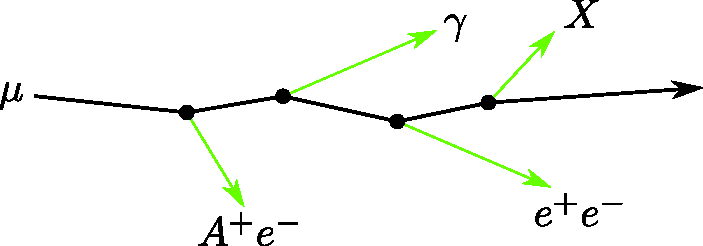
\includegraphics[width=0.7\textwidth]{images/muon_path.pdf}}

\definecolor{LightCyan}{rgb}{0.88,1,1}
\definecolor{LightRed}{rgb}{1,0.88,1}
\definecolor{LightGreen}{rgb}{1,1,0.88}

\begin{document}

\maketitle

\begin{frame}{Motivation}

\begin{figure}
    \begin{figure}[ht]
        \begin{minipage}[b]{0.4\linewidth}
            \centering
            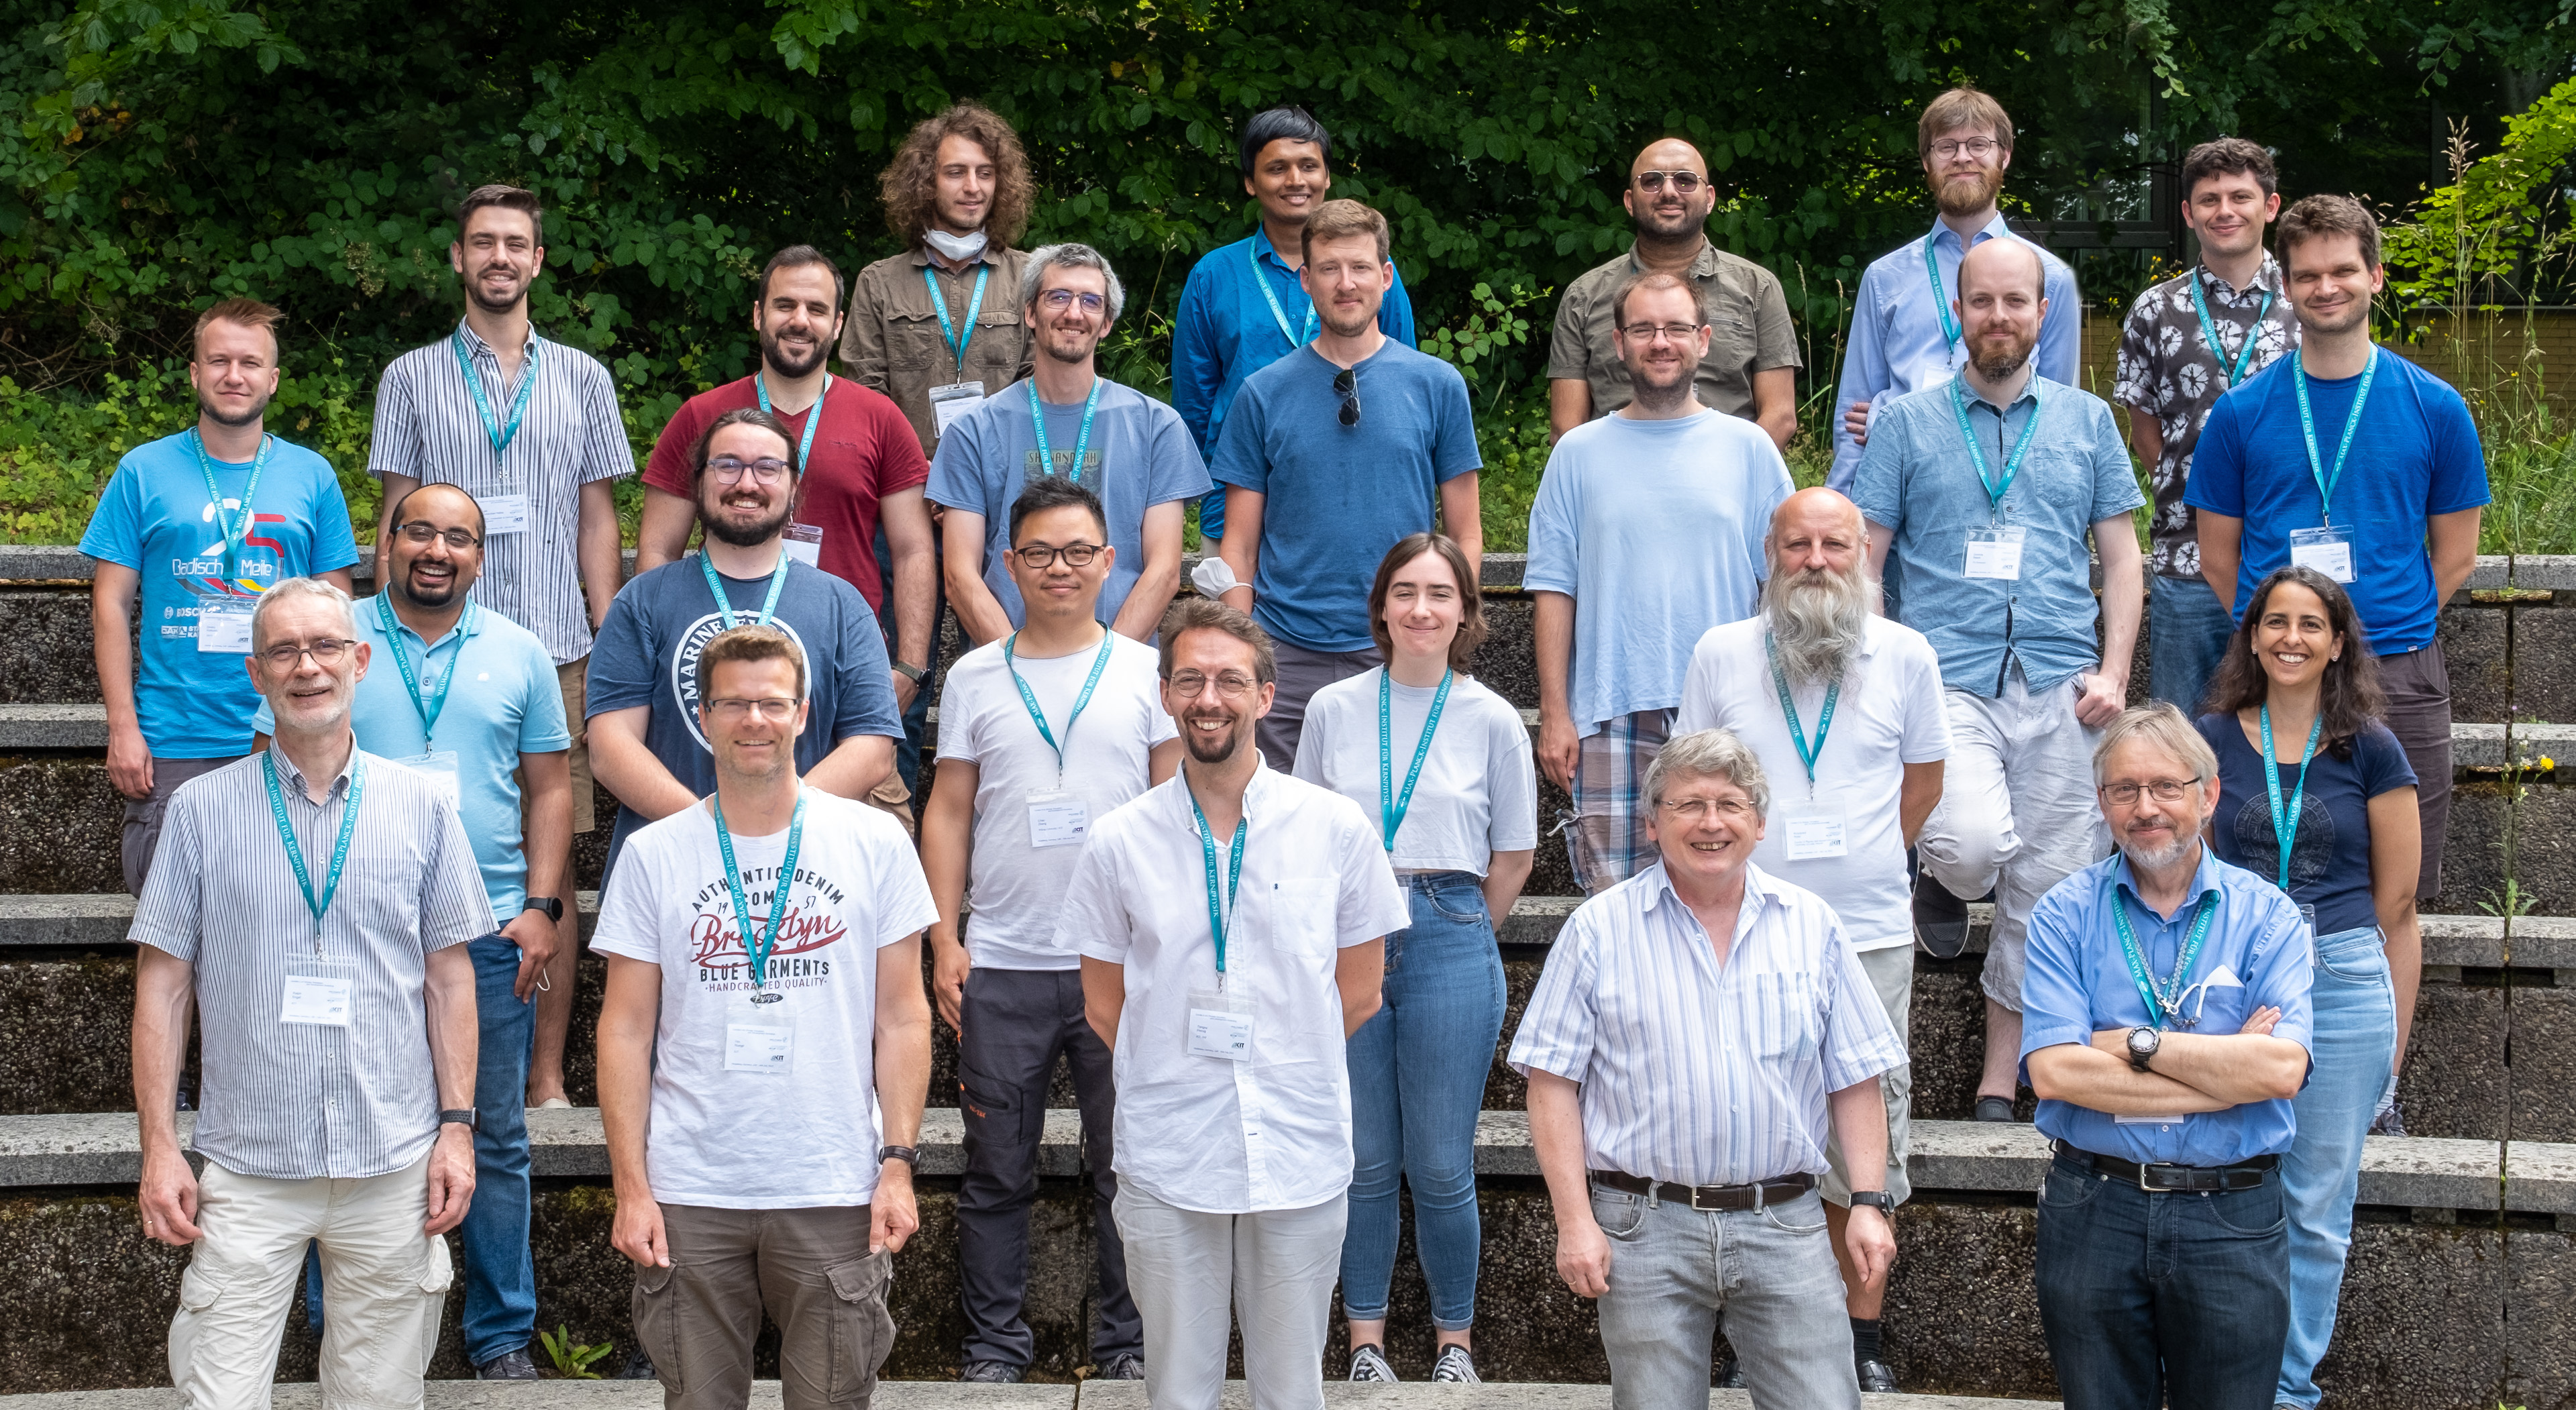
\includegraphics[width=\textwidth]{images/photo_2022.jpg}
            \caption*{CORSIKA 8 Workshop 2022}
            \label{fig:a}
        \end{minipage}
        \begin{minipage}[t]{0.15\linewidth}
          \vspace{-25mm}
          \centering
          \Huge\textbf{\rightarrow}
        \end{minipage}        
        \begin{minipage}[b]{0.4\linewidth}
            \centering
            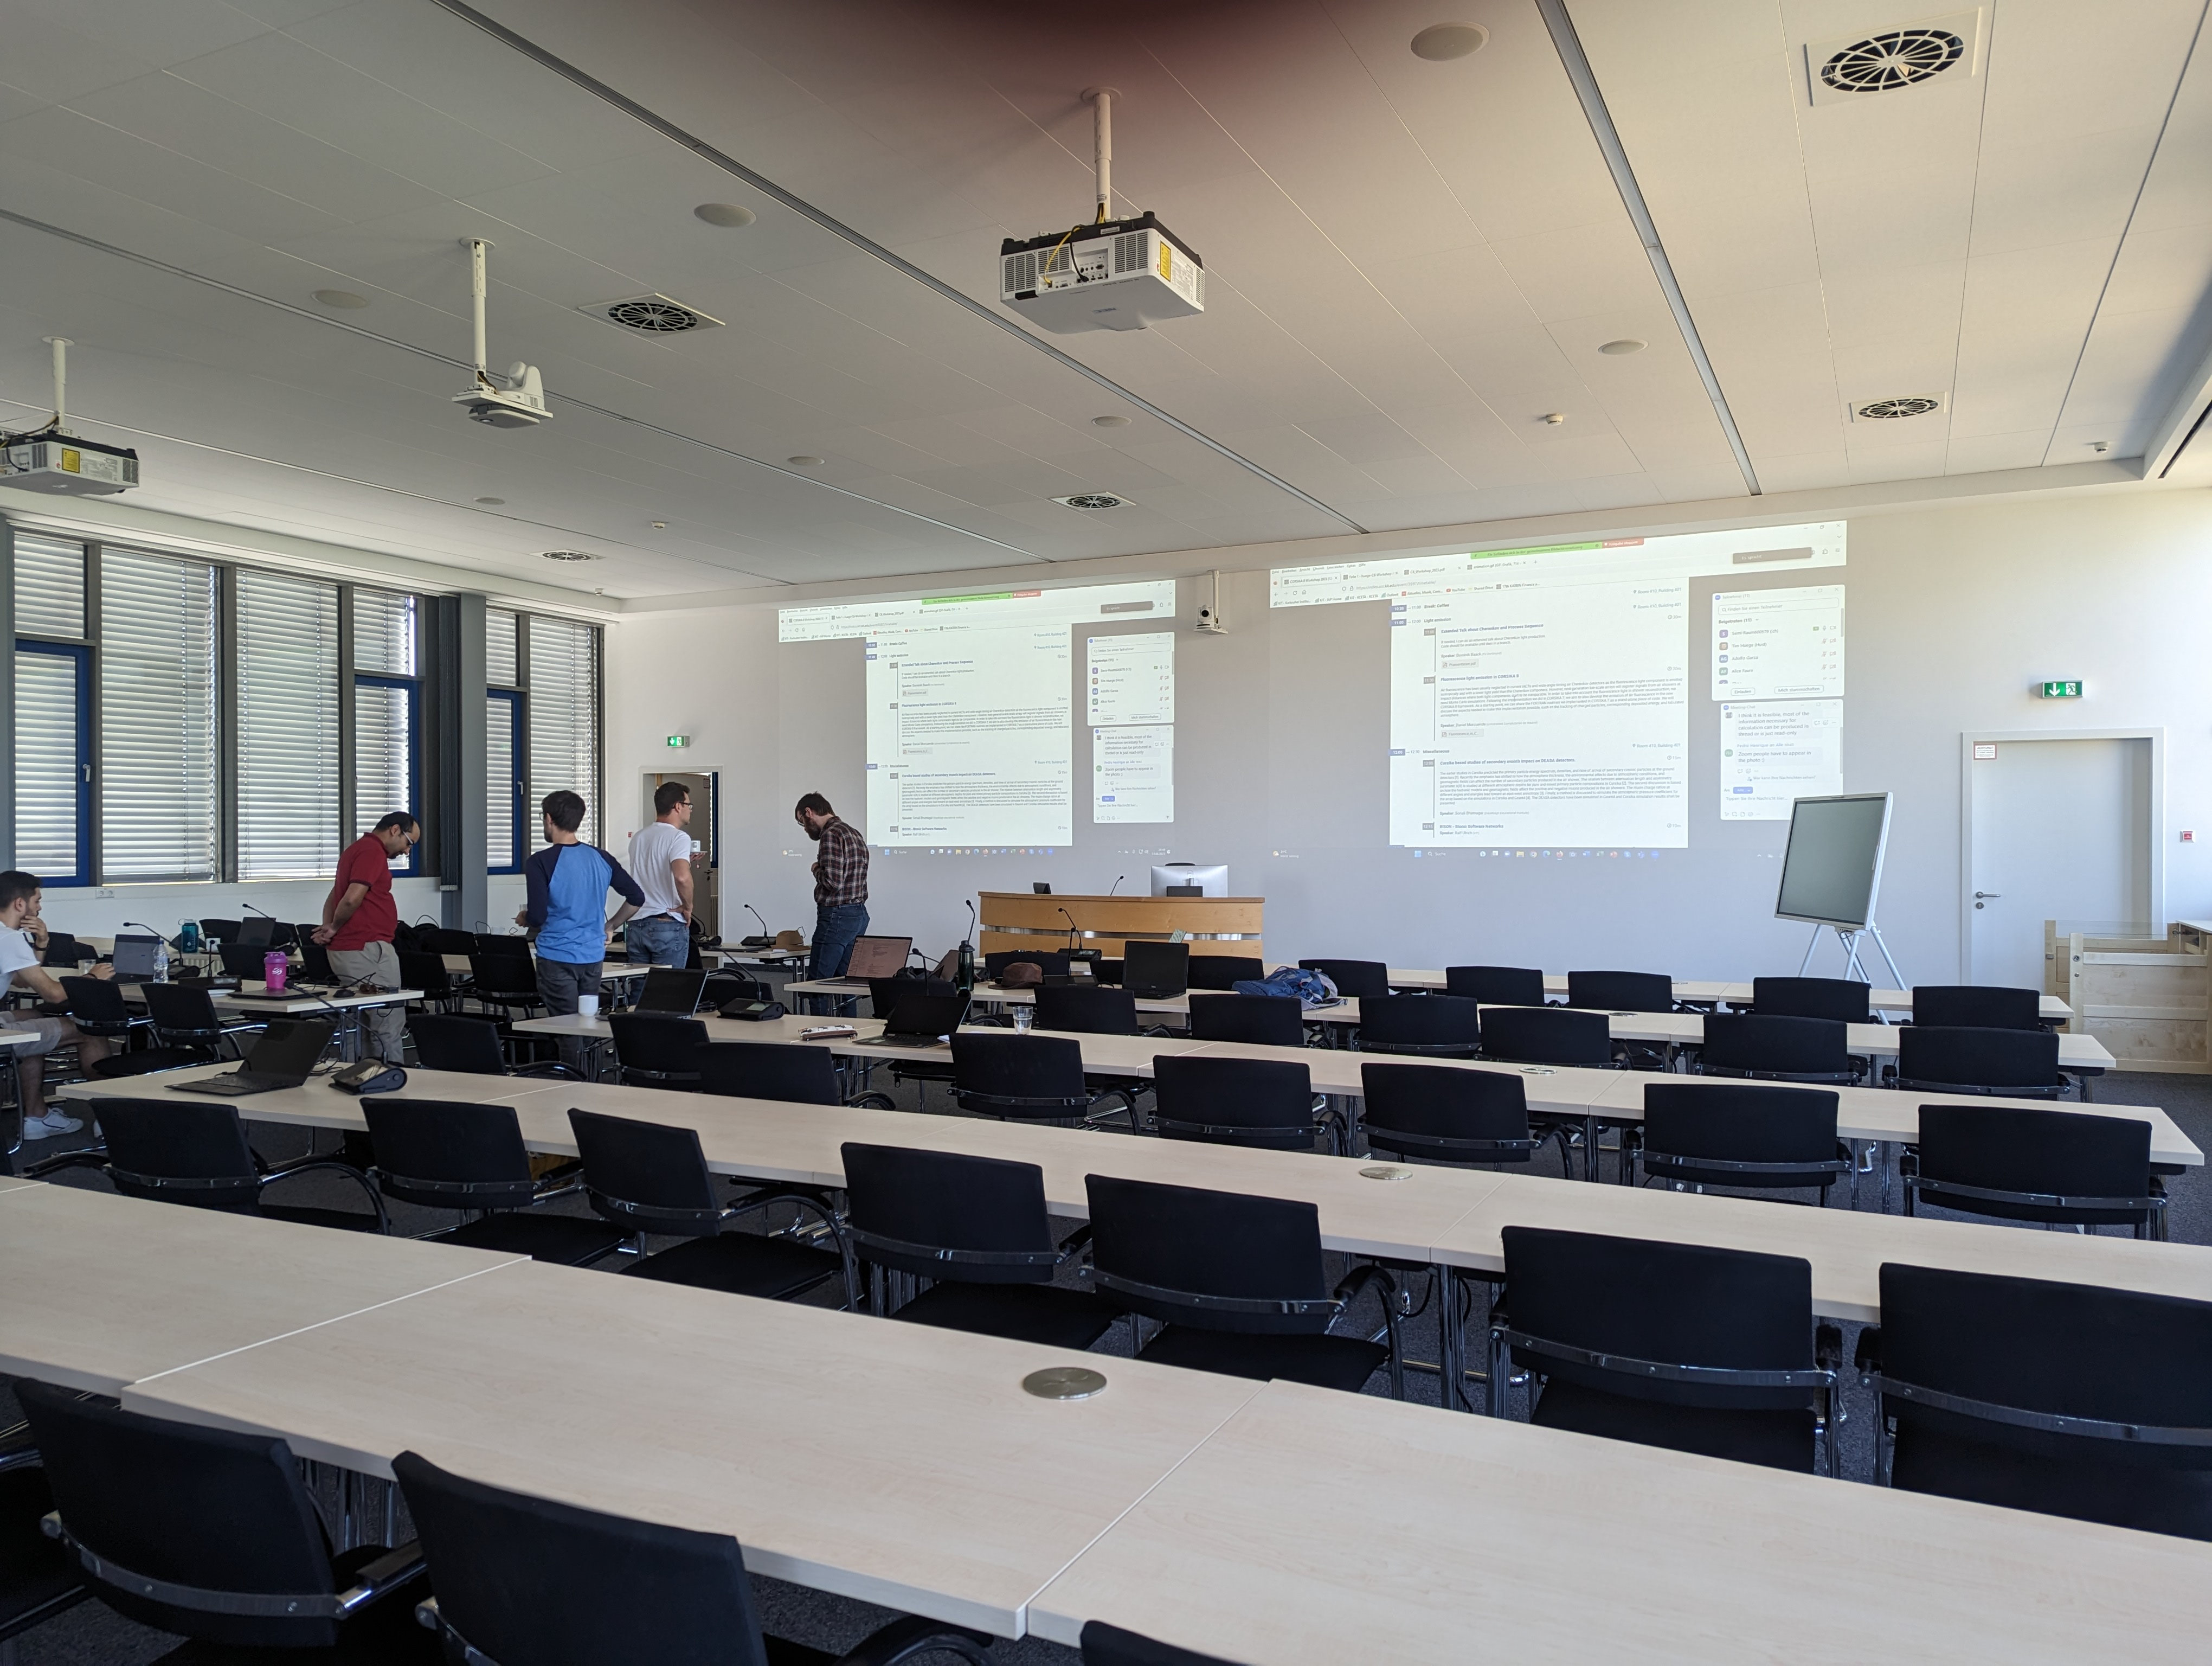
\includegraphics[width=\textwidth]{images/photo_2023_prelim.jpg}
            \caption*{CORSIKA 8 Workshop 2023}
            \label{fig:b}
        \end{minipage}
    \end{figure}
\end{figure}

  \begin{itemize}
    \item Idea of this talk: Present updates of EM simulations within CORSIKA~8 since the last workshop
    \begin{itemize}
        \item[$\rightarrow$] However, it is exceptionally hard to present one full year of development in one talk
        \item[$\rightarrow$] I'll try to focus on some of the most important updates
    \end{itemize}
  \end{itemize}
\end{frame}

\begin{frame}[plain,c,noframenumbering]
  \begin{center}
    \Huge Conclusions from the 2022 workshop
  \end{center}
\end{frame}

\section{Conclusions from the 2022 workshop}


\begin{frame}

\textbf{Looking back at the 2022 workshop - Which problems within the EM component did we identify?}

    \begin{columns}[onlytextwidth]
        \begin{column}{0.5\textwidth}
            \begin{itemize}
              \item \textbf{CORSIKA~8 produces too many charged leptons (compared to CORSIKA~7)}
              \item \textbf{CORSIKA~8 showers tend to develop earlier}
              \item The charge excess within CORSIKA~8 is higher
              \item Lateral profiles don't agree, CORSIKA~8 particles are shifted towards the shower axis
            \end{itemize}
        \end{column}
        \begin{column}{0.5\textwidth}
            \begin{figure}
                \centering
                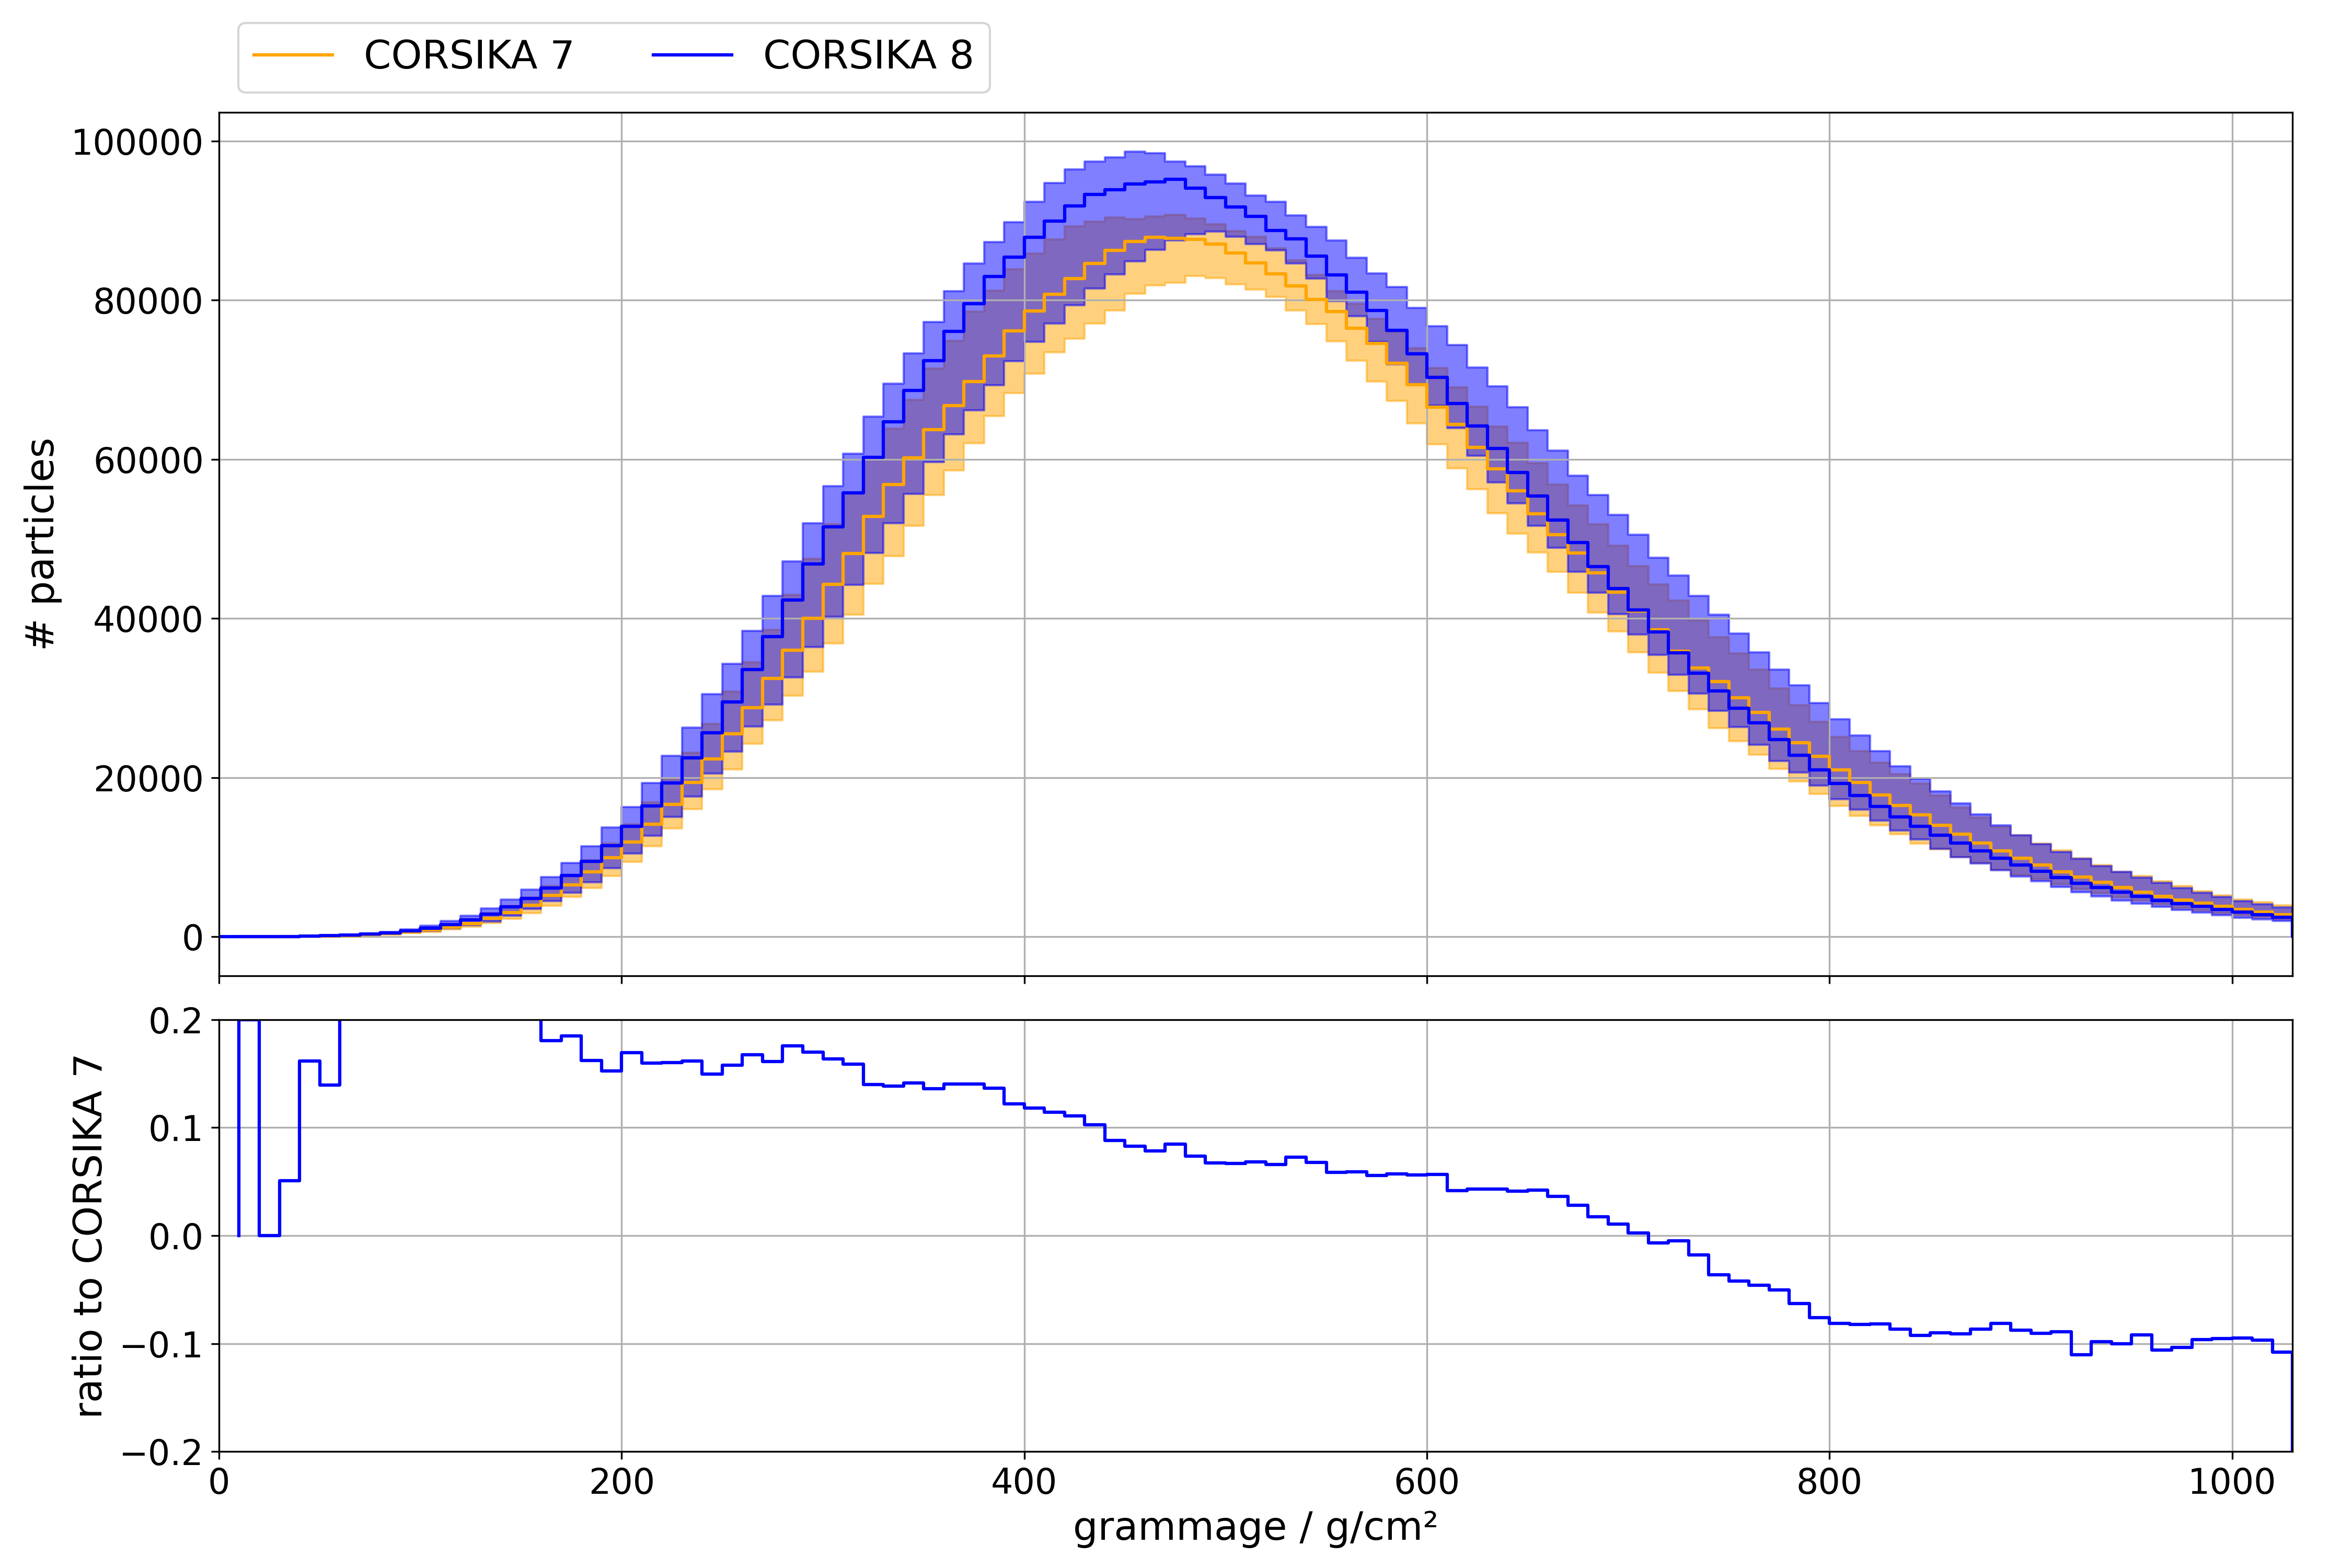
\includegraphics[width=0.95\textwidth]{plots/long_charged_2022.png}
                \caption{Longitudinal profile of charged particles in 100 \si{\tera\electronvolt} $e^-$ showers, 2022 workshop.}
            \end{figure}
        \end{column}
    \end{columns}
\end{frame}

\begin{frame}

\textbf{Looking back at the 2022 workshop - Which problems within the EM component did we identify?}

    \begin{columns}[onlytextwidth]
        \begin{column}{0.5\textwidth}
            \begin{itemize}
              \item CORSIKA~8 produces too many charged leptons (compared to CORSIKA~7)
              \item CORSIKA~8 showers tend to develop earlier
              \item \textbf{The charge excess within CORSIKA~8 is higher}
              \item Lateral profiles don't agree, CORSIKA~8 particles are shifted towards the shower axis
            \end{itemize}
        \end{column}
        \begin{column}{0.5\textwidth}
            \begin{figure}
                \centering
                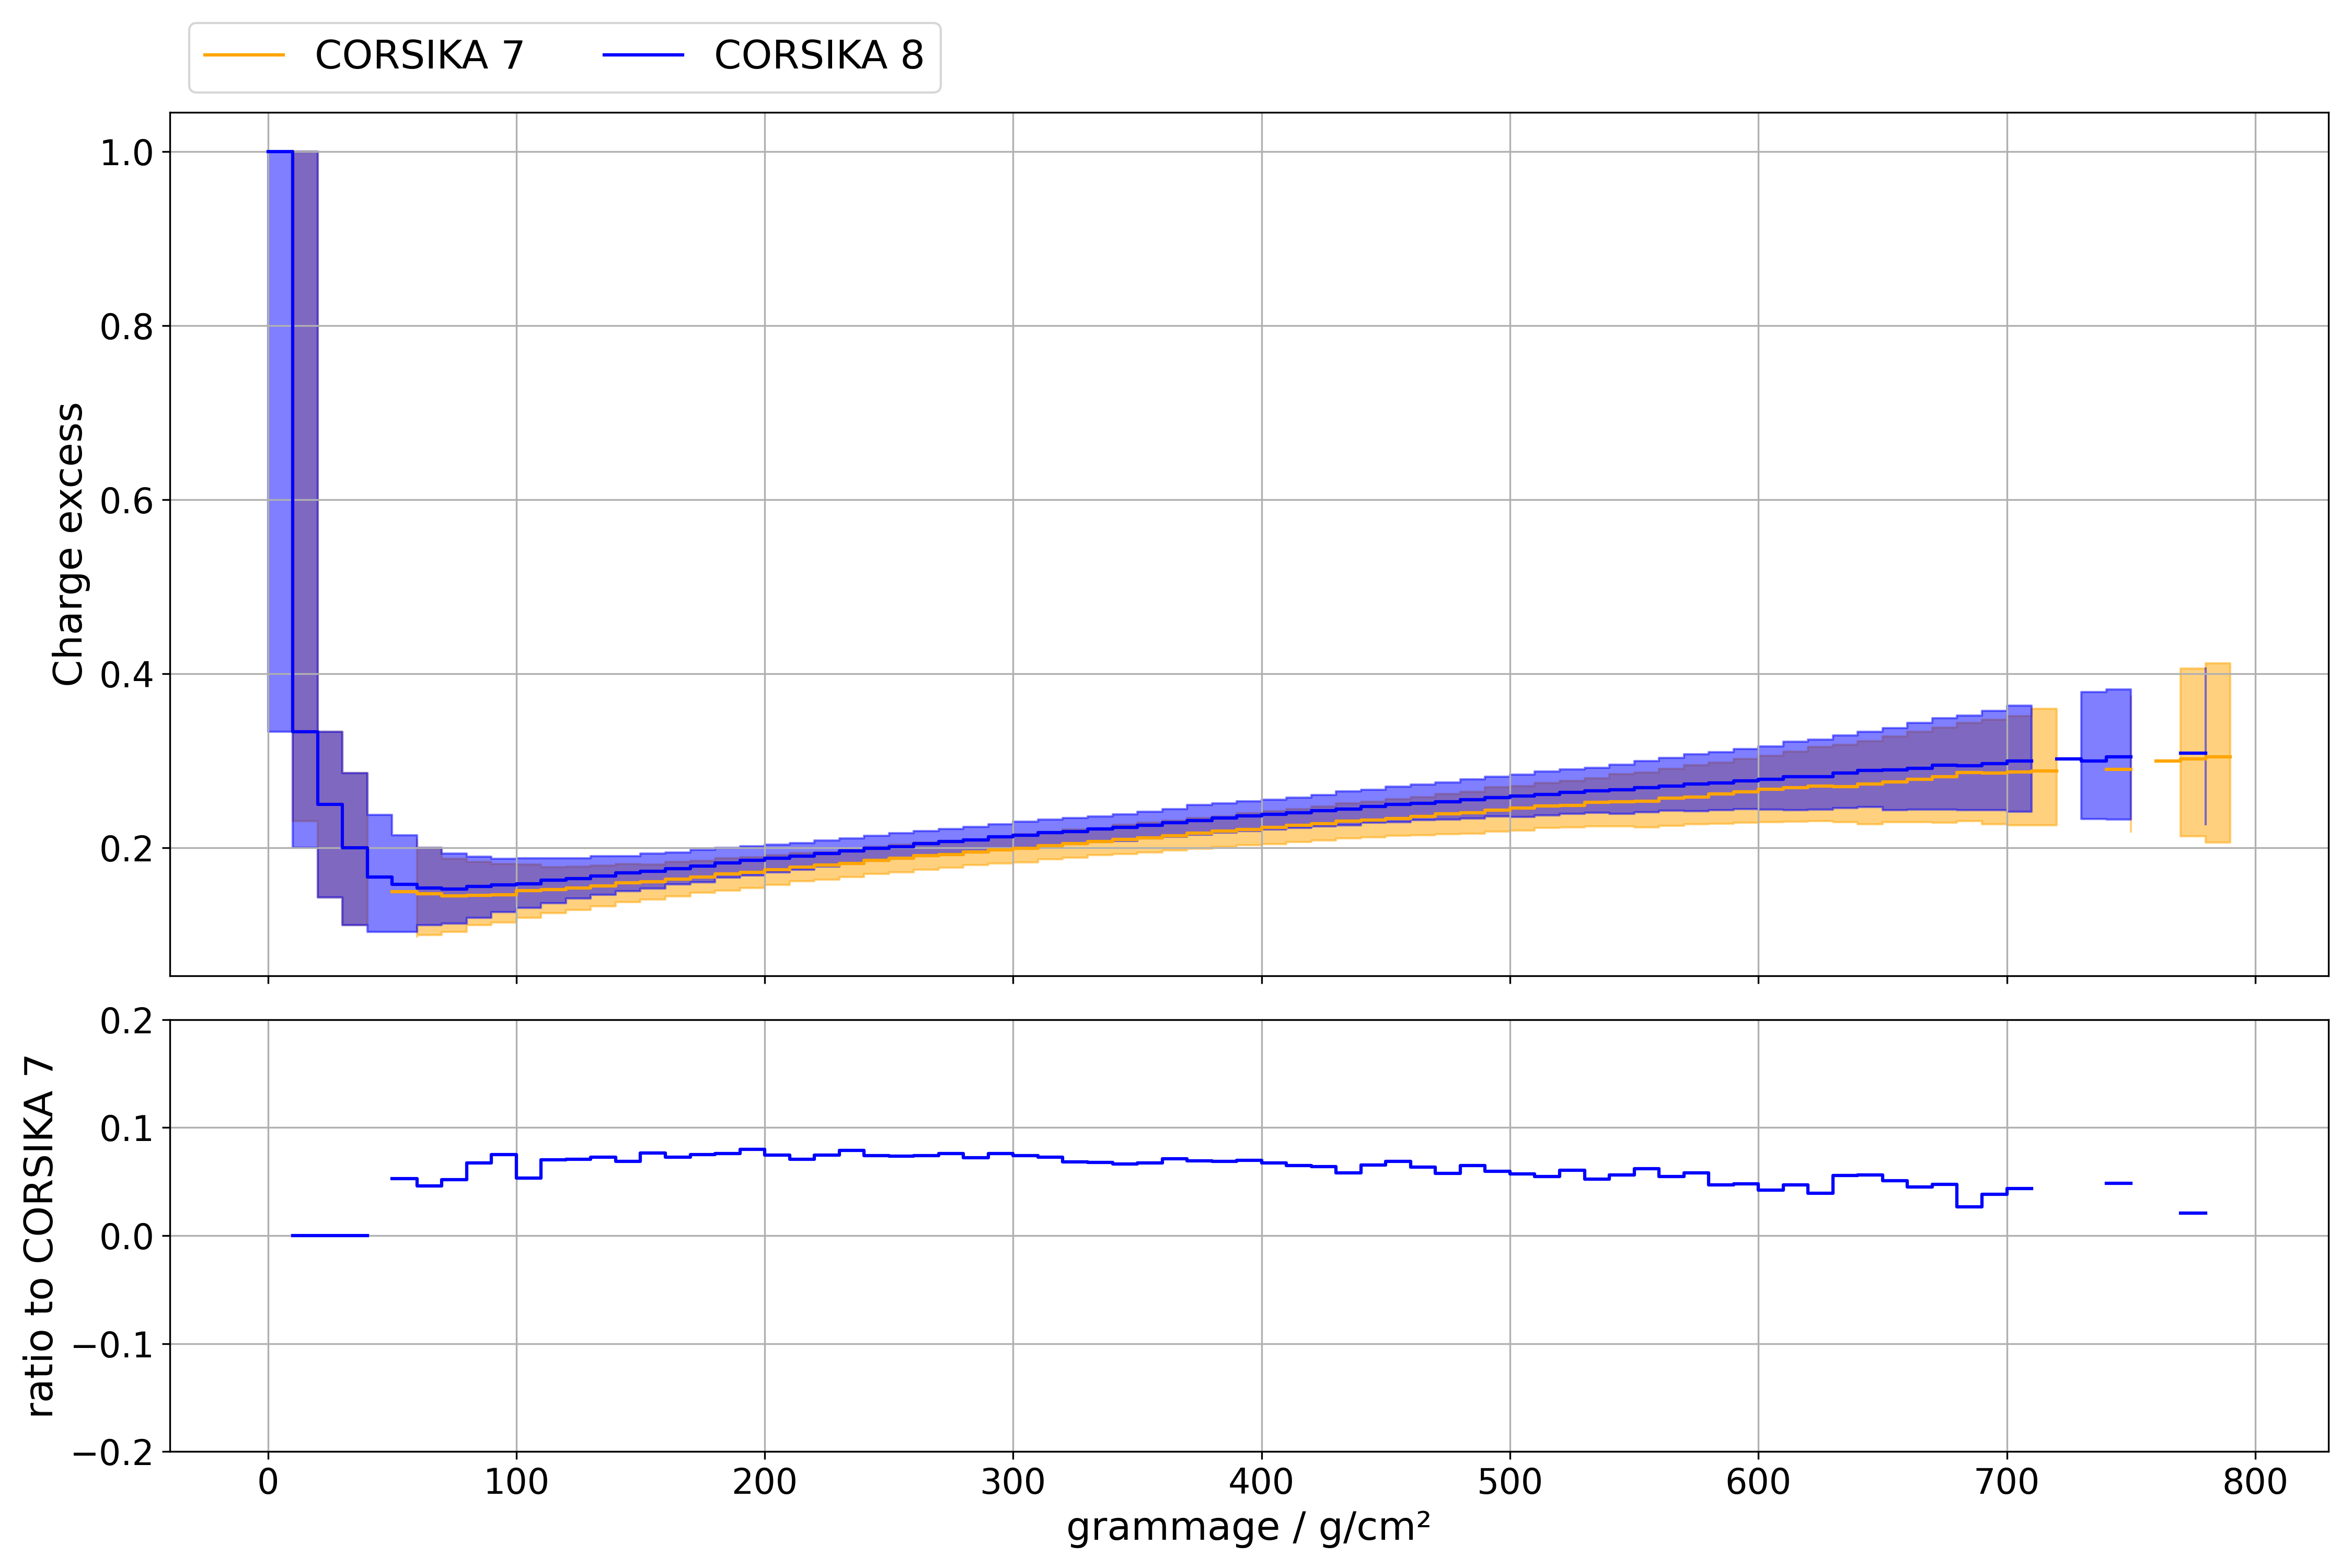
\includegraphics[width=0.95\textwidth]{plots/charge_excess_2022.png}
                \caption{Longitudinal charge excess ($\frac{N_{e^-} - N_{e^+}}{N_{e^-} + N_{e^+}}$) in 1 \si{\tera\electronvolt} showers, 2022 workshop.}
            \end{figure}
        \end{column}
    \end{columns}
\end{frame}


\begin{frame}

\textbf{Looking back at the 2022 workshop - Which problems within the EM component did we identify?}

    \begin{columns}[onlytextwidth]
        \begin{column}{0.5\textwidth}
            \begin{itemize}
              \item CORSIKA~8 produces too many charged leptons (compared to CORSIKA~7)
              \item CORSIKA~8 showers tend to develop earlier
              \item The charge excess within CORSIKA~8 is higher
              \item \textbf{Lateral profiles don't agree, CORSIKA~8 particles are shifted towards the shower axis}
            \end{itemize}
        \end{column}
        \begin{column}{0.5\textwidth}
            \begin{figure}
                \centering
                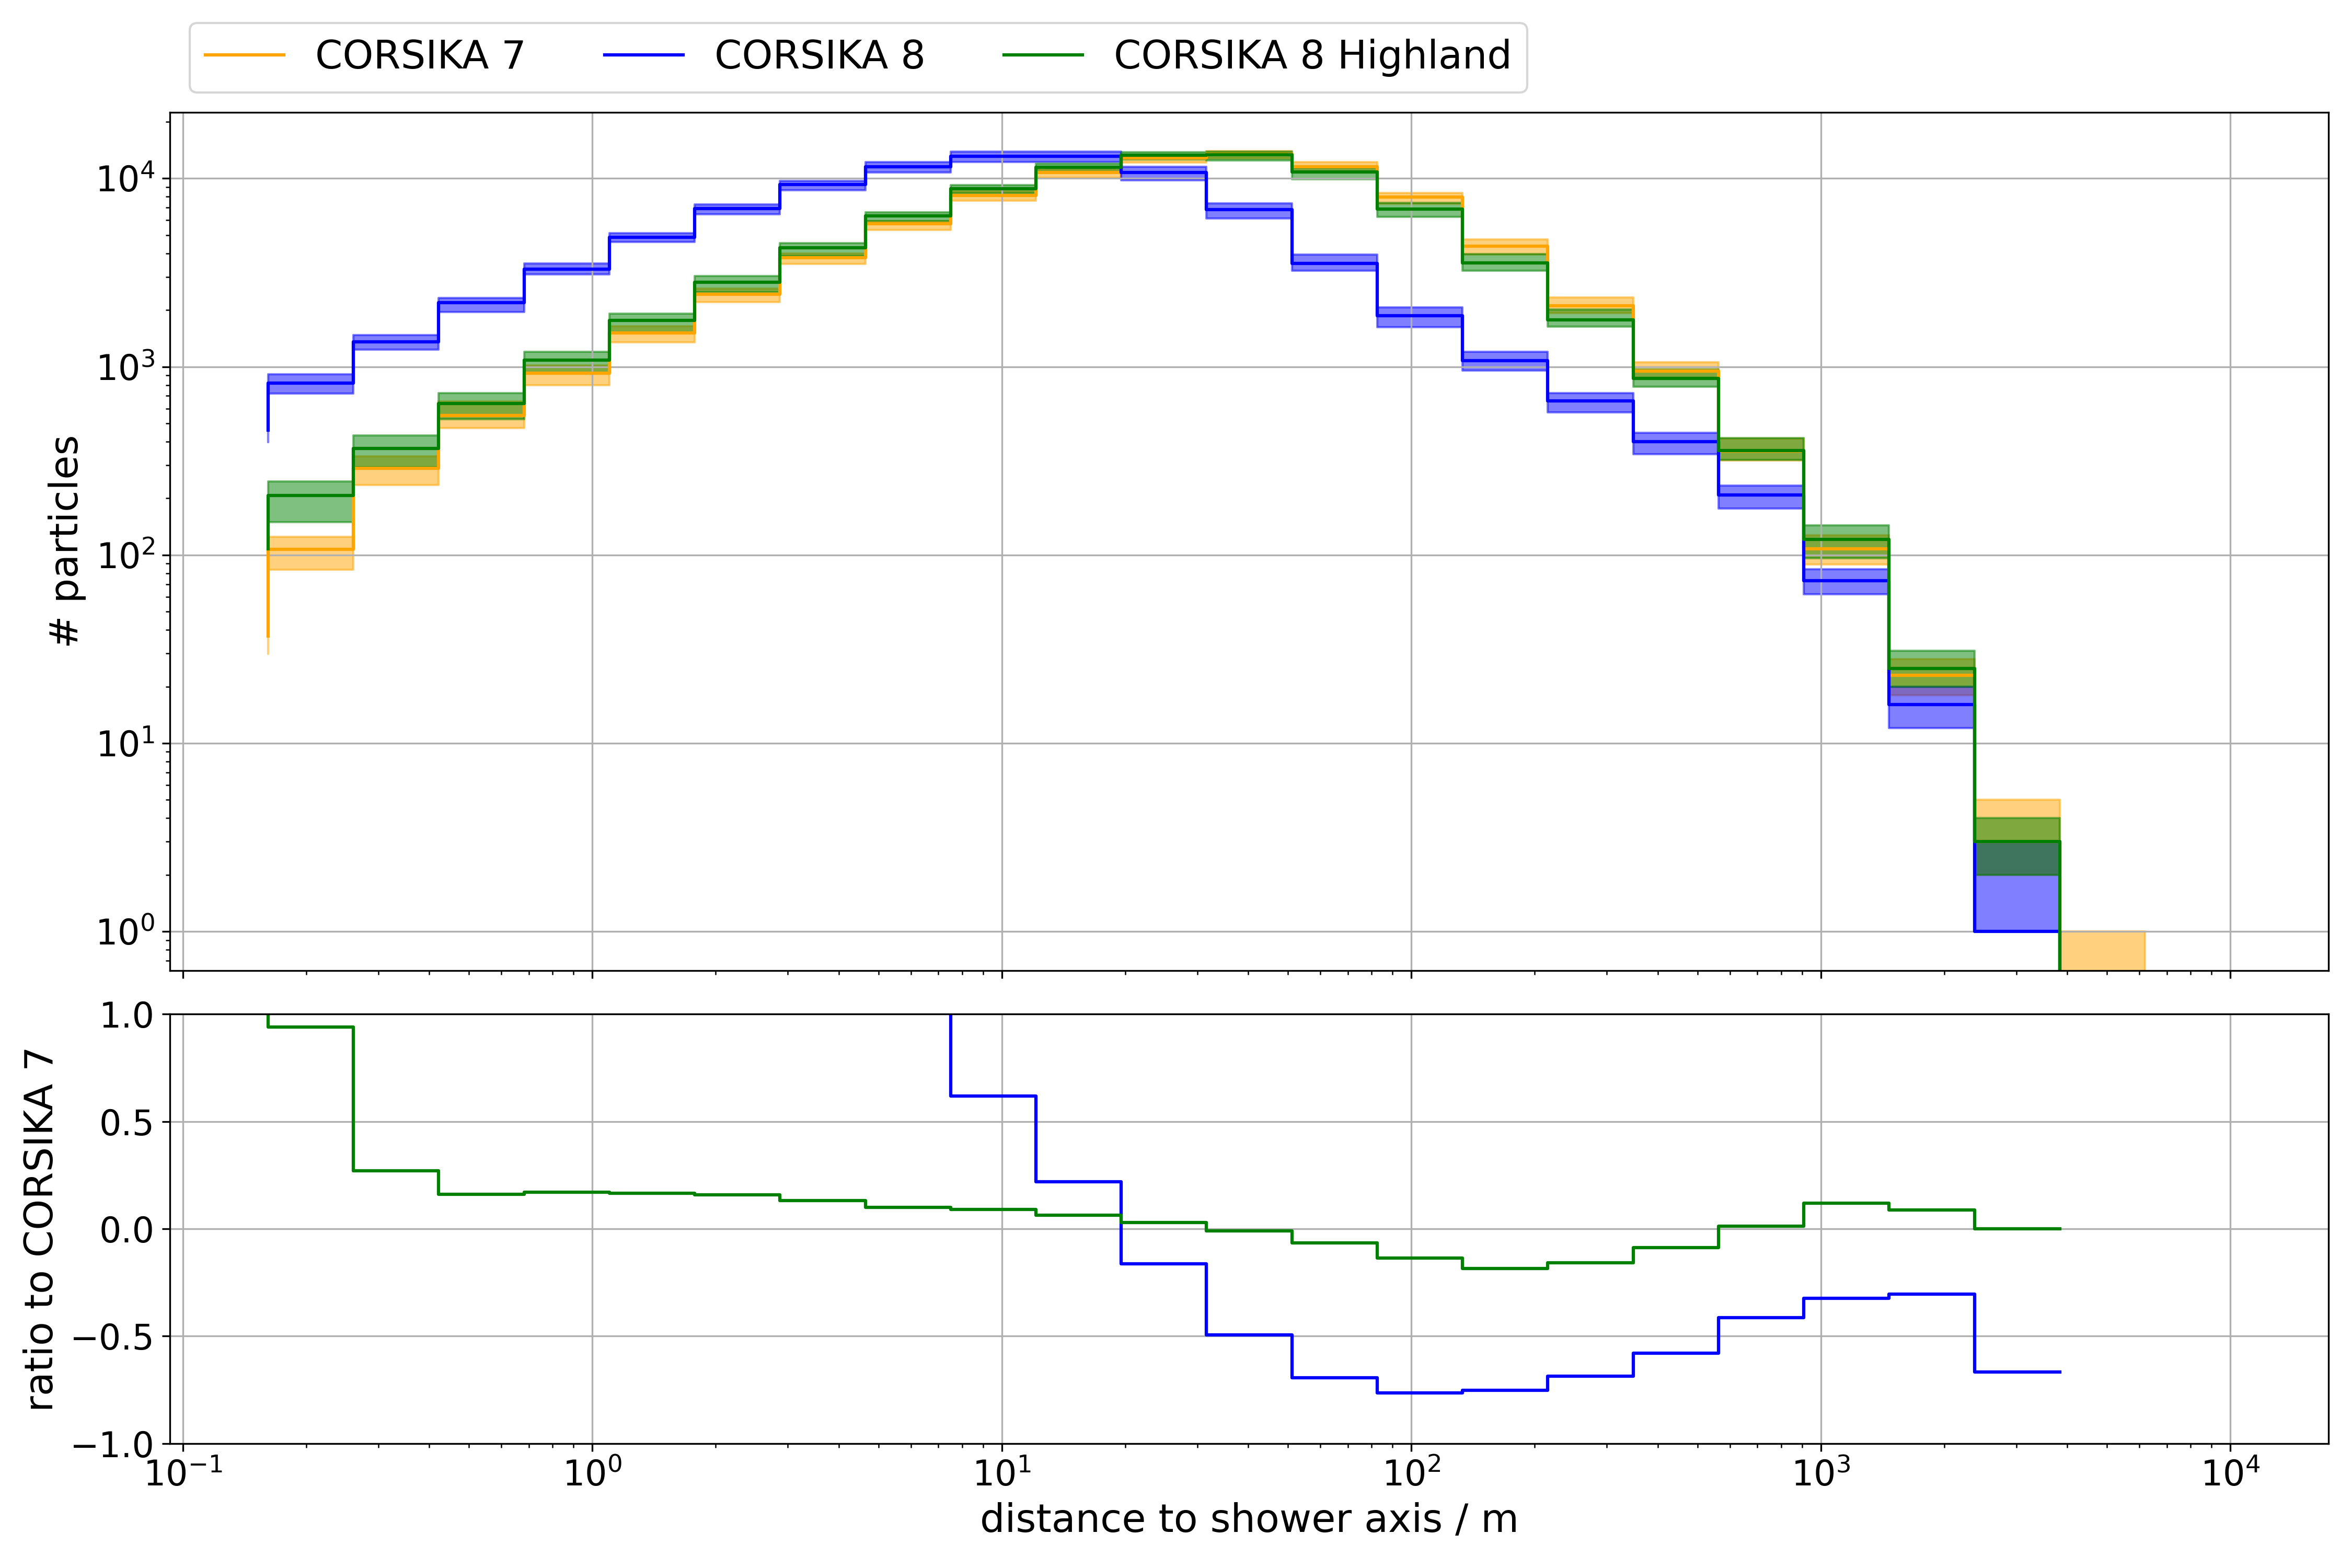
\includegraphics[width=0.95\textwidth]{plots/lateral_r_charged_2022.png}
                \caption{Lateral profiles for 100 \si{\tera\electronvolt} showers at $X_\text{max}$, 2022 workshop.}
            \end{figure}
        \end{column}
    \end{columns}
\end{frame}


\begin{frame}[plain,c,noframenumbering]
  \begin{center}
    \Huge Bugfixes and improvements
  \end{center}
\end{frame}

\section{Bugfixes and improvements}

\begin{frame}
\textbf{"Cascade bug"}
\vspace{5mm}
\begin{itemize}
  \item Prior to the 2022 workshop, we discovered an issue within the basic \texttt{Cascade} algorithm of CORSIKA~8
  \item It was not clear at which position of a continuous step energies are evaluated
  \begin{itemize}
    \item[$\rightarrow$] Cross sections weren't evaluated at the correct energies
    \item[$\rightarrow$] Multiple scattering was not (correctly) taken into account
  \end{itemize}
  \item \textbf{Huge} effort by Nikos and Maximilian to fix this issue ($\approx$ 6 months of development) \emoji{muscle}
  \begin{itemize}
    \item[$\rightarrow$] Implementation of a \texttt{Step} object, which collects all incremental changes to a particle state from all continuous processes
    \item[$\rightarrow$] It is now much clearer what continuous processes are doing
  \end{itemize}
\end{itemize}
\end{frame}


\begin{frame}
  \textbf{Influence on longitudinal profiles}
  \vspace{5mm}
  \begin{itemize}
    \item The fix of the \texttt{Cascade} algorithm means that cross sections are evaluated correctly now
    \item Furthermore, we have adapted the kinematic limits of the bremsstrahlung cross section
    \begin{itemize}
      \item[$\rightarrow$] Better agreement with EGS4 cross sections, for details see \href{https://github.com/tudo-astroparticlephysics/PROPOSAL/pull/308}{here}
    \end{itemize}
    \item We have fixed a bug where the difference of ionization between $e^-$ and $e^+$ was treated incorrectly by PROPOSAL
  \end{itemize}
\end{frame}


\begin{frame}

  \textbf{Influence on longitudinal profiles}
  \vspace{5mm}

    \begin{columns}[onlytextwidth]
        \begin{column}{0.4\textwidth}
            \begin{itemize}
              \item Charge excess in very good agreement ($< \SI{1}{\percent}$) with CORSIKA~7 now
            \end{itemize}
        \end{column}
        \begin{column}{0.6\textwidth}
            \begin{figure}
                \centering
                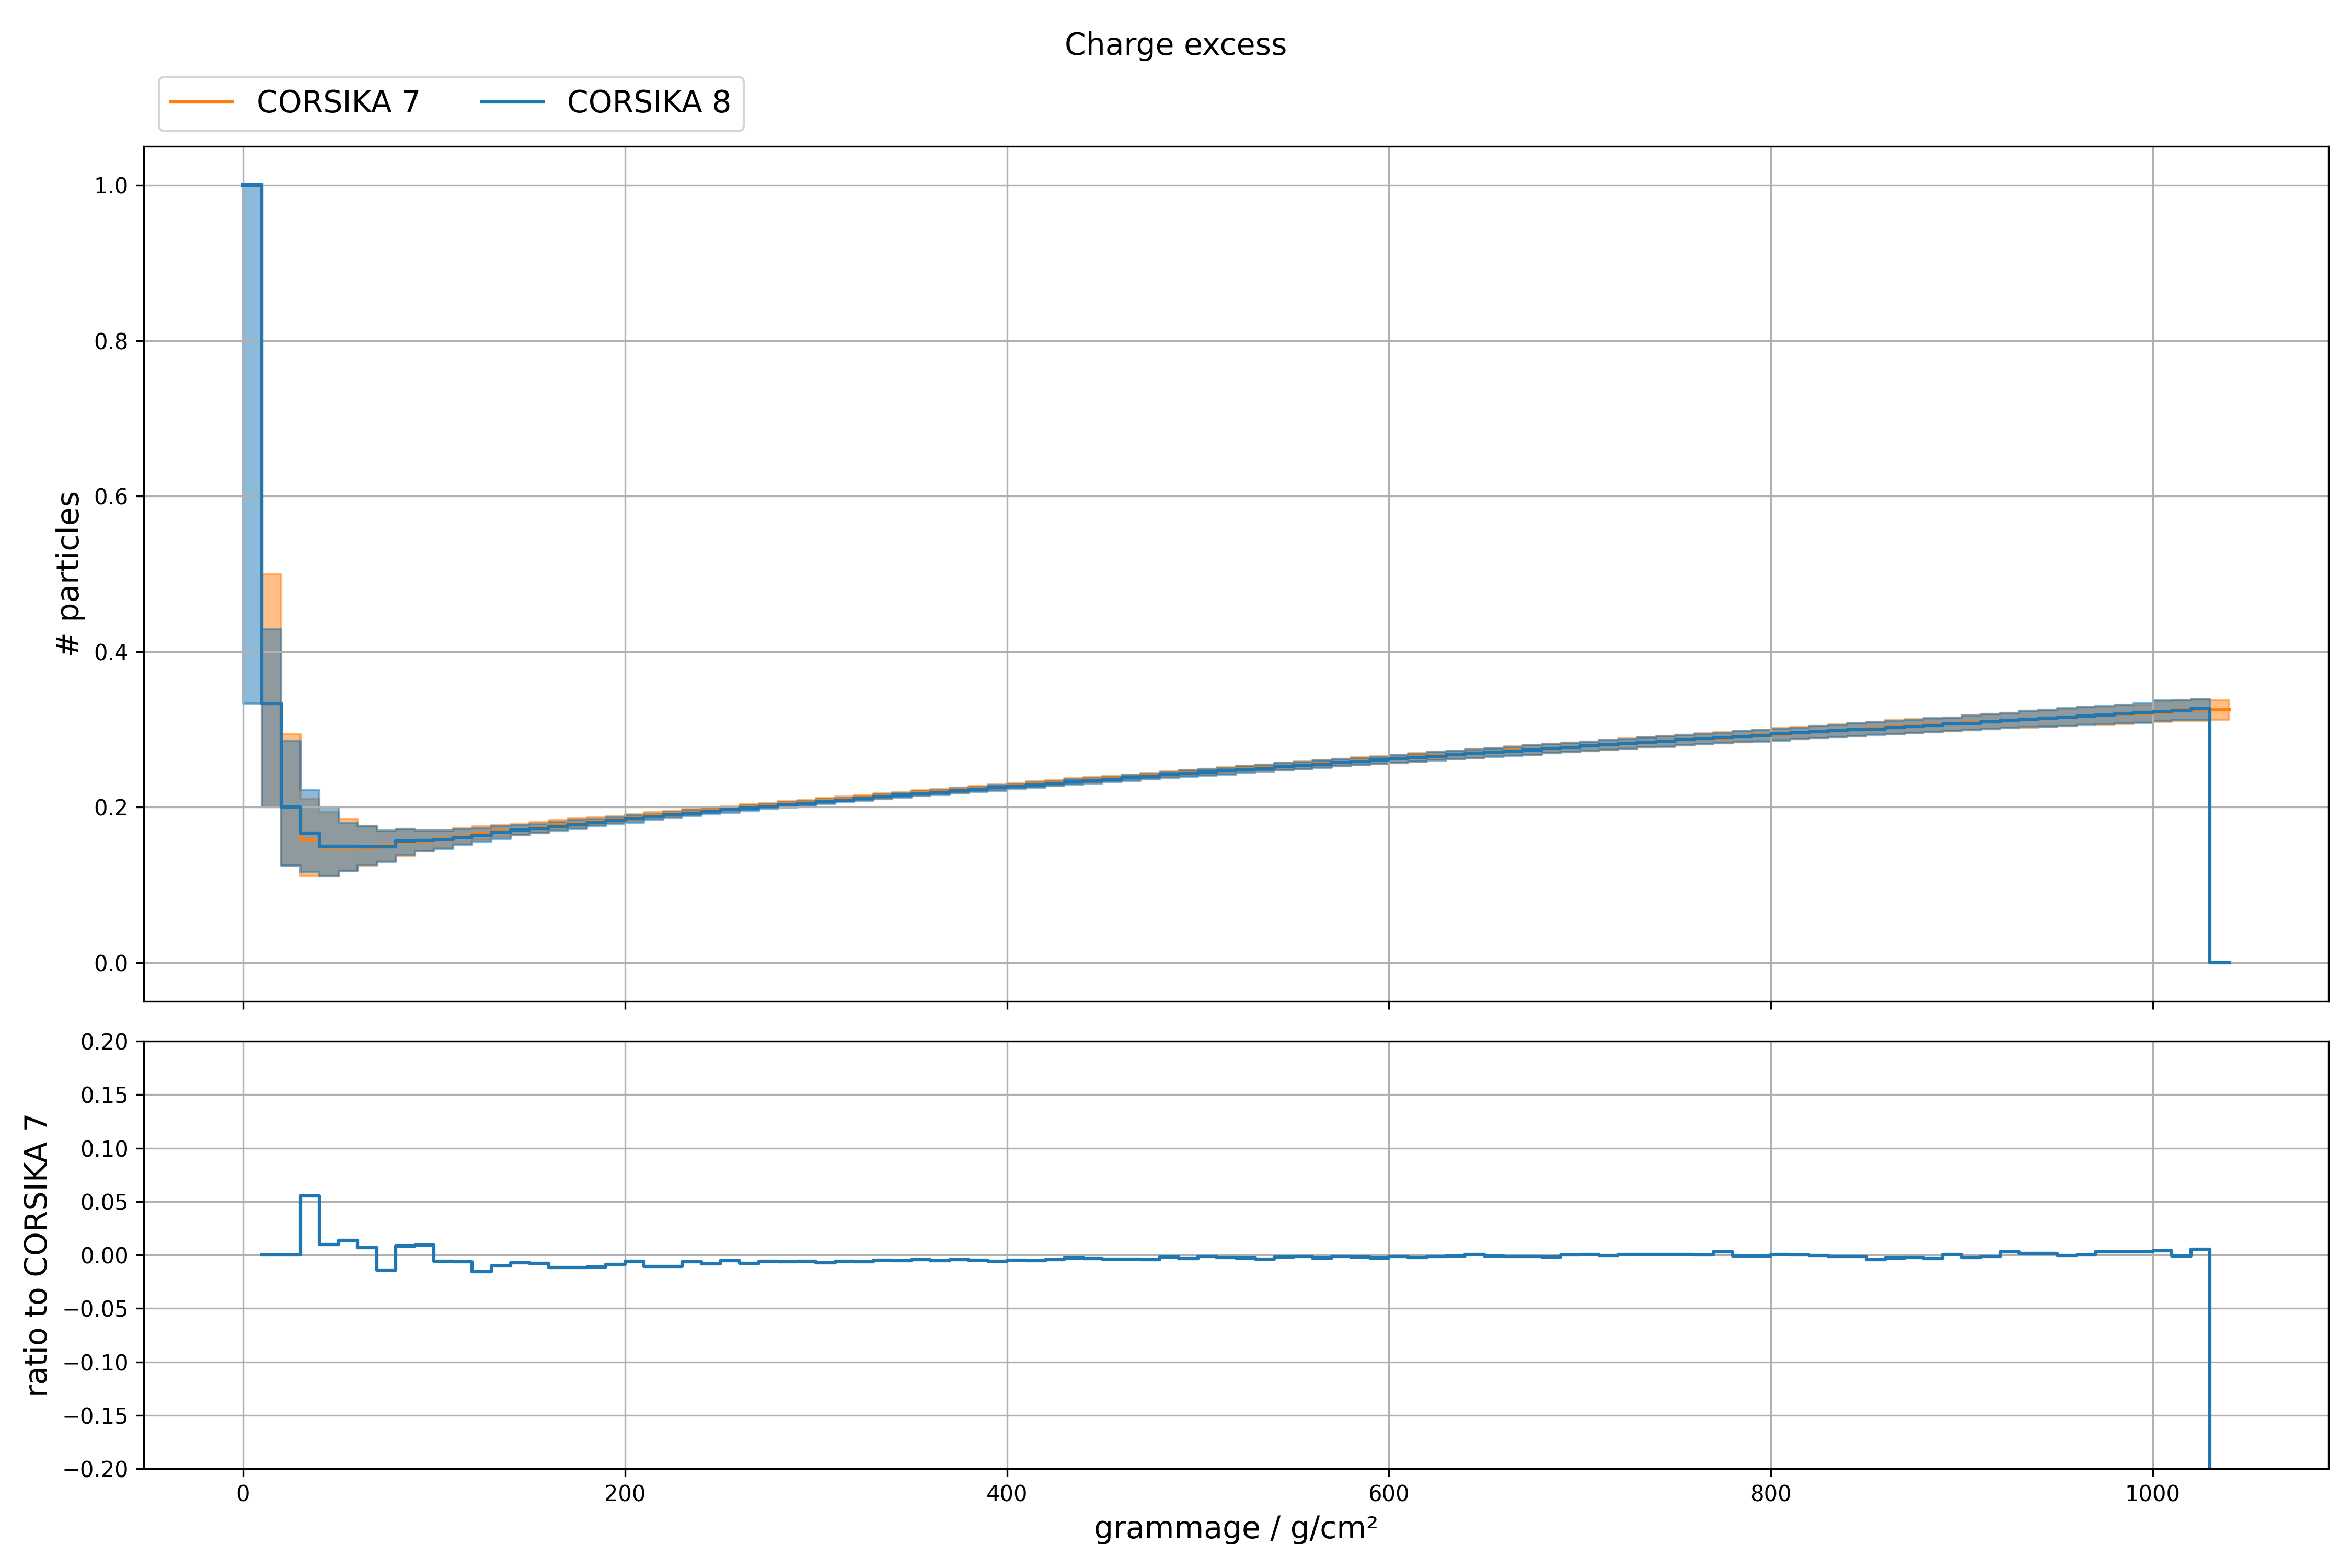
\includegraphics[width=0.95\textwidth]{plots/charge_excess_2023.png}
                \caption{Longitudinal charge excess ($\frac{N_{e^-} - N_{e^+}}{N_{e^-} + N_{e^+}}$) in 100 \si{\tera\electronvolt} showers, current status.}
            \end{figure}
        \end{column}
    \end{columns}
\end{frame}


\begin{frame}

  \textbf{Influence on longitudinal profiles}
  \vspace{5mm}

    \begin{columns}[onlytextwidth]
        \begin{column}{0.4\textwidth}
            \begin{itemize}
              \item Better agreement concerning the overall number of charged particles
              \begin{itemize}
                \item[$\rightarrow$] However, CORSIKA~8 showers still develop earlier compared to CORSIKA~7 
              \end{itemize}
            \end{itemize}
        \end{column}
        \begin{column}{0.6\textwidth}
            \begin{figure}
                \centering
                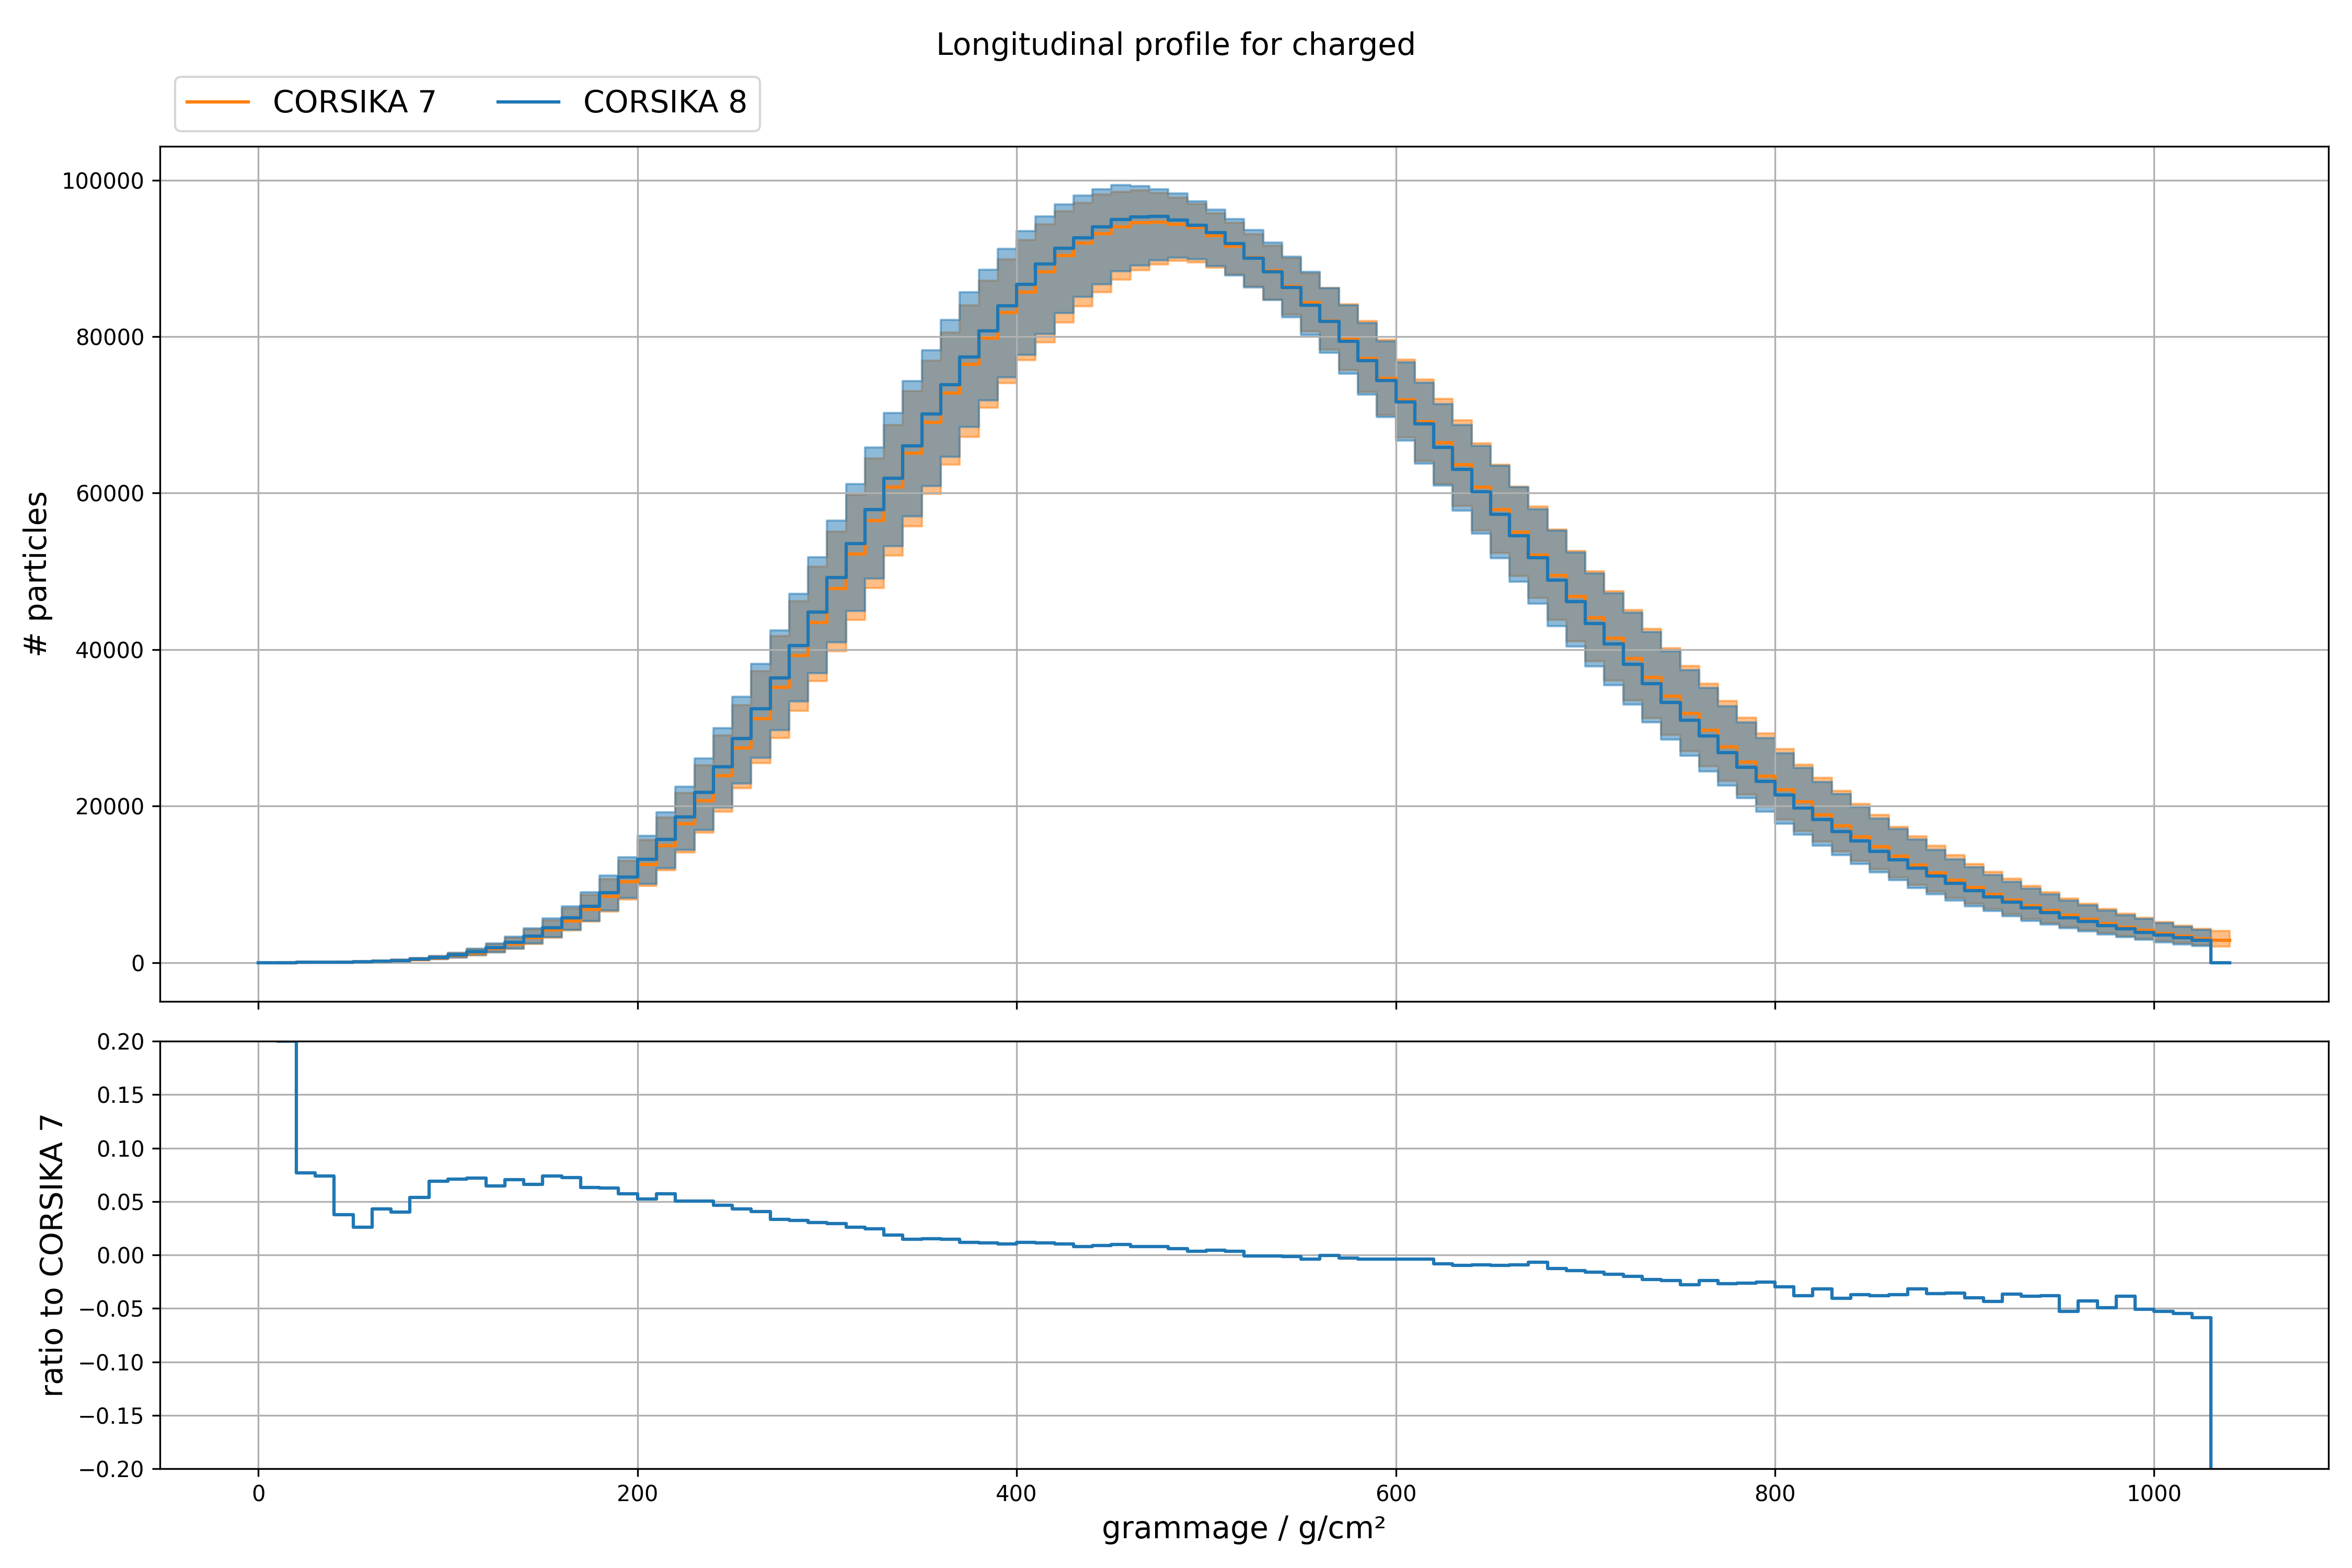
\includegraphics[width=0.95\textwidth]{plots/long_charged_2023.png}
                \caption{Longitudinal profile of charged particles in 100 \si{\tera\electronvolt} showers, current status.}
            \end{figure}
        \end{column}
    \end{columns}
\end{frame}


\begin{frame}

  \textbf{Influence on longitudinal profiles}
  \vspace{5mm}

    \begin{columns}[onlytextwidth]
        \begin{column}{0.4\textwidth}
            \begin{itemize}
              \item Looking at the longitudinal profile of photons, we are missing photons compared to CORSIKA~7
            \end{itemize}
        \end{column}
        \begin{column}{0.6\textwidth}
            \begin{figure}
                \centering
                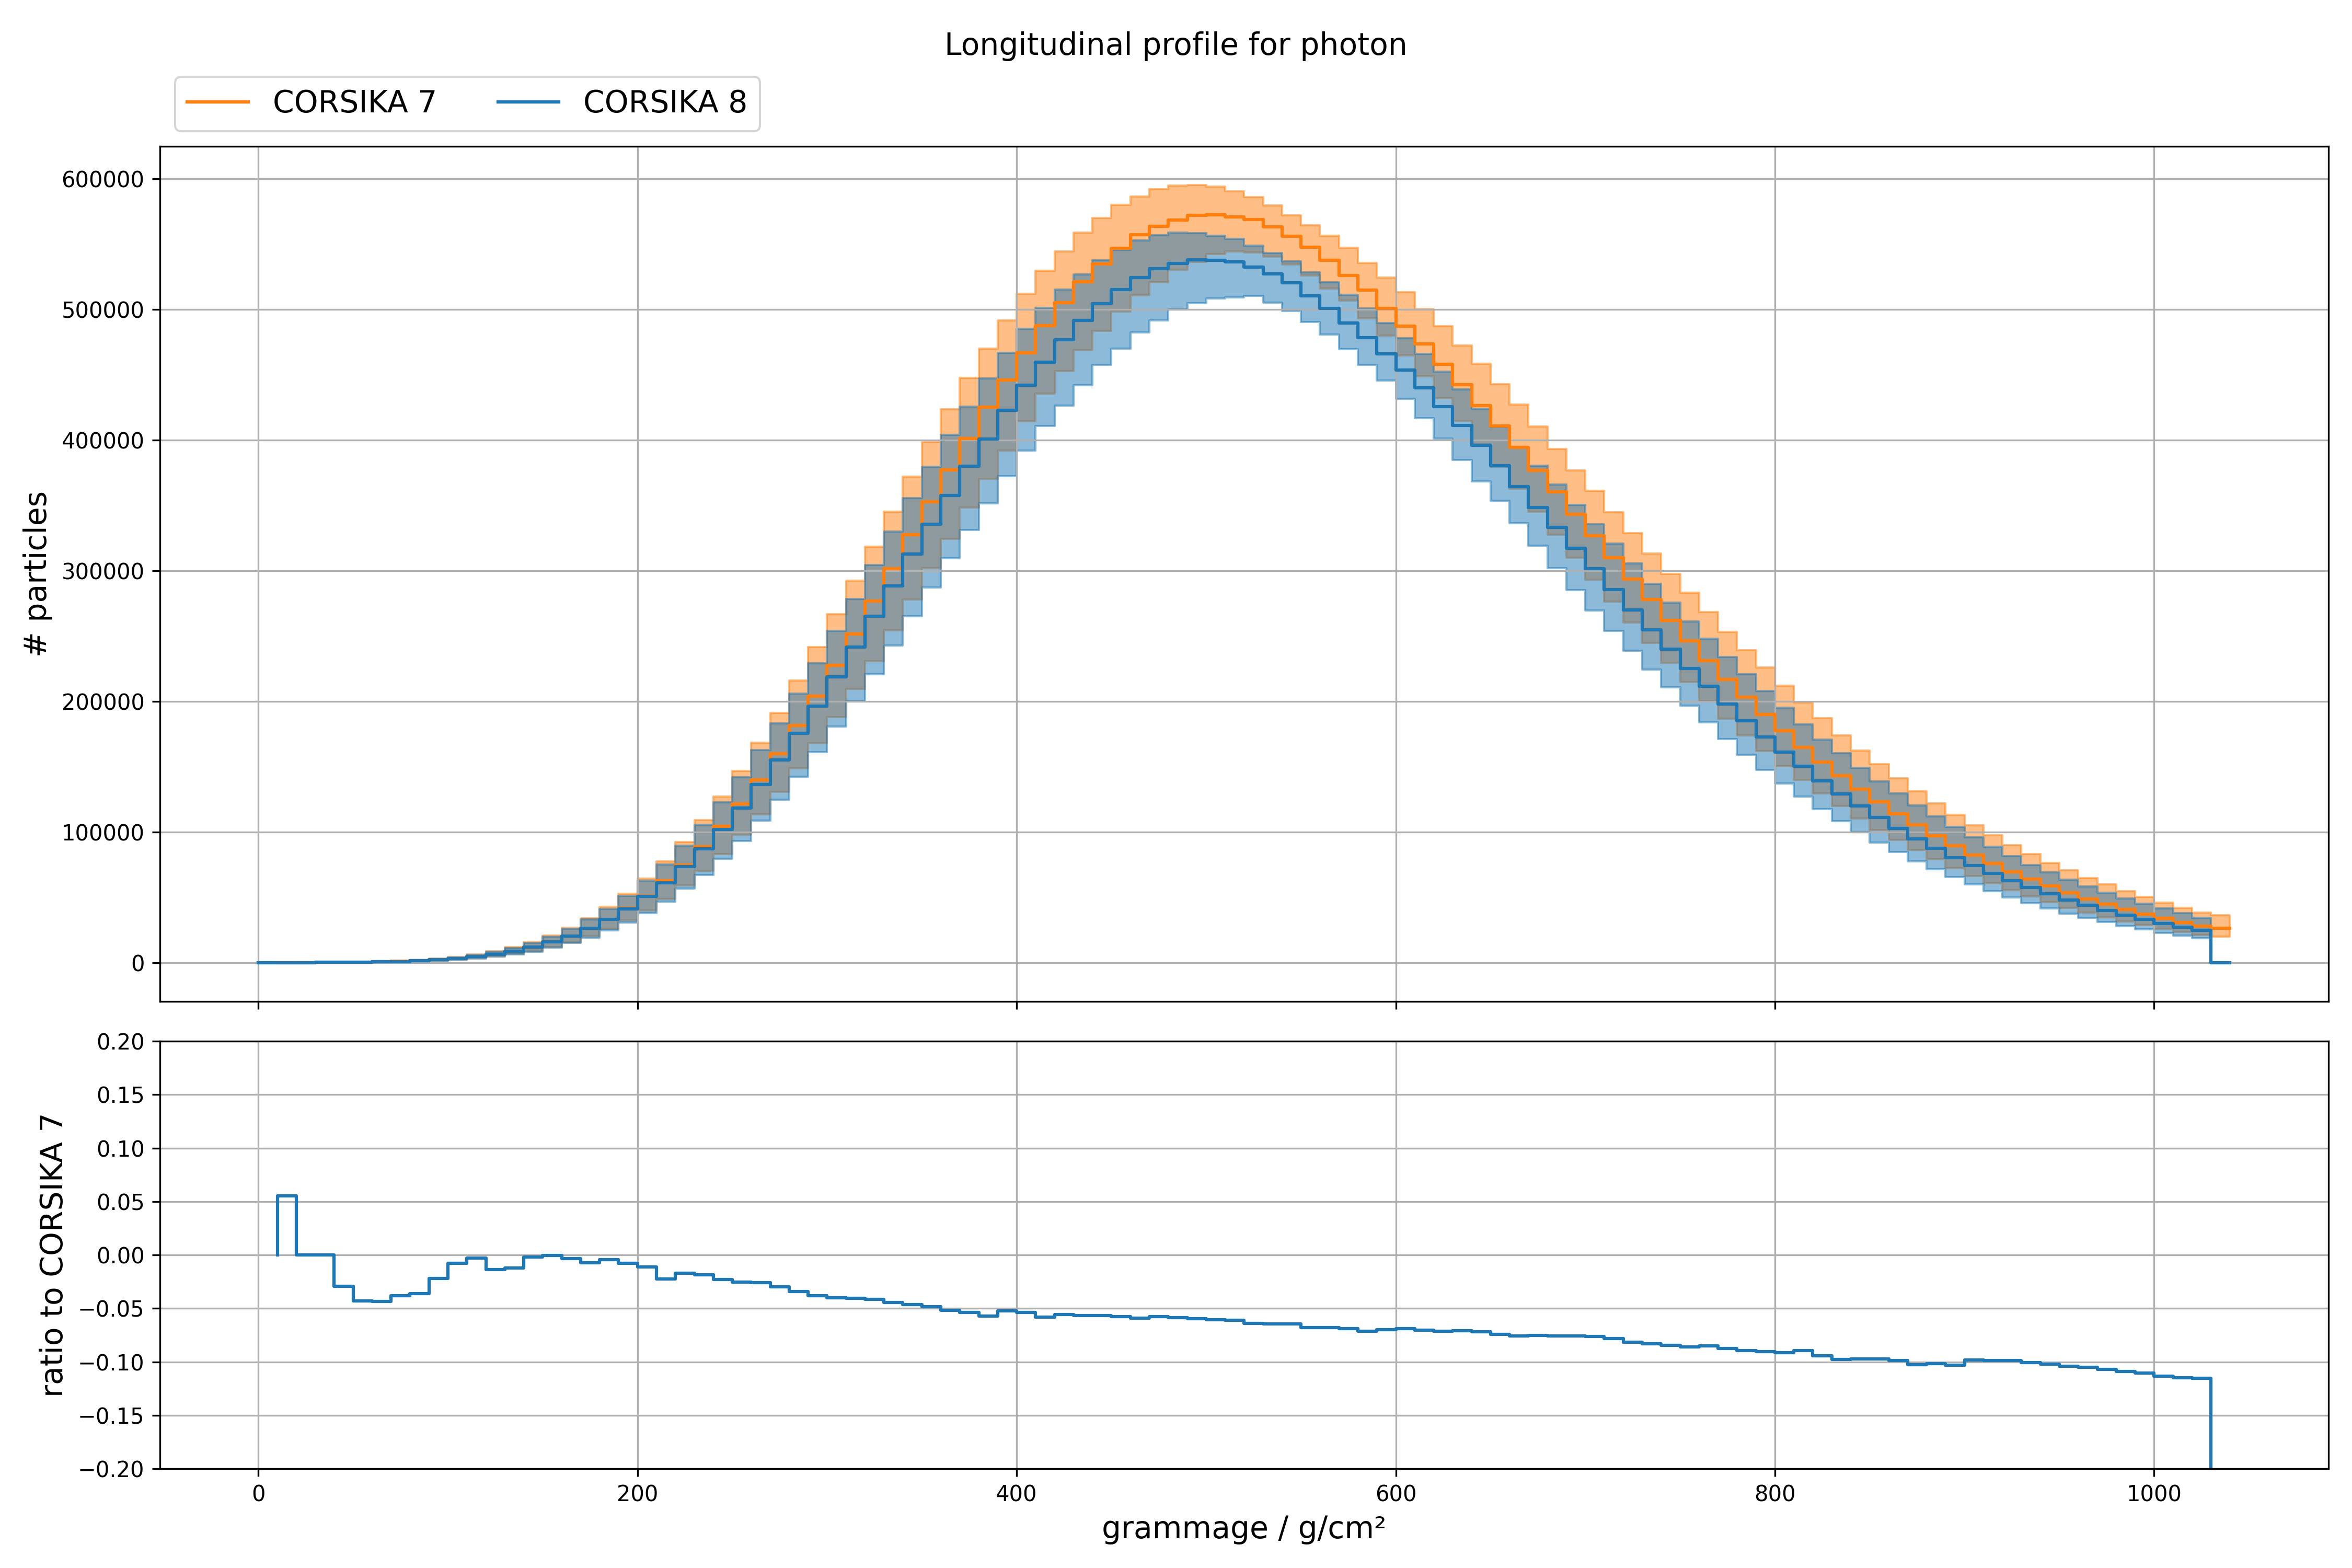
\includegraphics[width=0.95\textwidth]{plots/long_photon_2023_full.png}
                \caption{Longitudinal profile of photons in 100 \si{\tera\electronvolt} showers, current status.}
            \end{figure}
        \end{column}
    \end{columns}
\end{frame}

\begin{frame}
  \textbf{Influence on longitudinal profiles}
  \vspace{5mm}
    \begin{columns}[onlytextwidth]
        \begin{column}{0.4\textwidth}
            \begin{itemize}
              \item Looking at the longitudinal profile of photons, we are missing photons compared to CORSIKA~7
              \begin{itemize}
                \item[$\rightarrow$] If we only look at photons with enegies above $\SI{20}{\mega\electronvolt}$, the particle number agrees
                \item[$\rightarrow$] This means that low-energy photons are missing
              \end{itemize}
            \end{itemize}
        \end{column}
        \begin{column}{0.6\textwidth}
            \begin{figure}
                \centering
                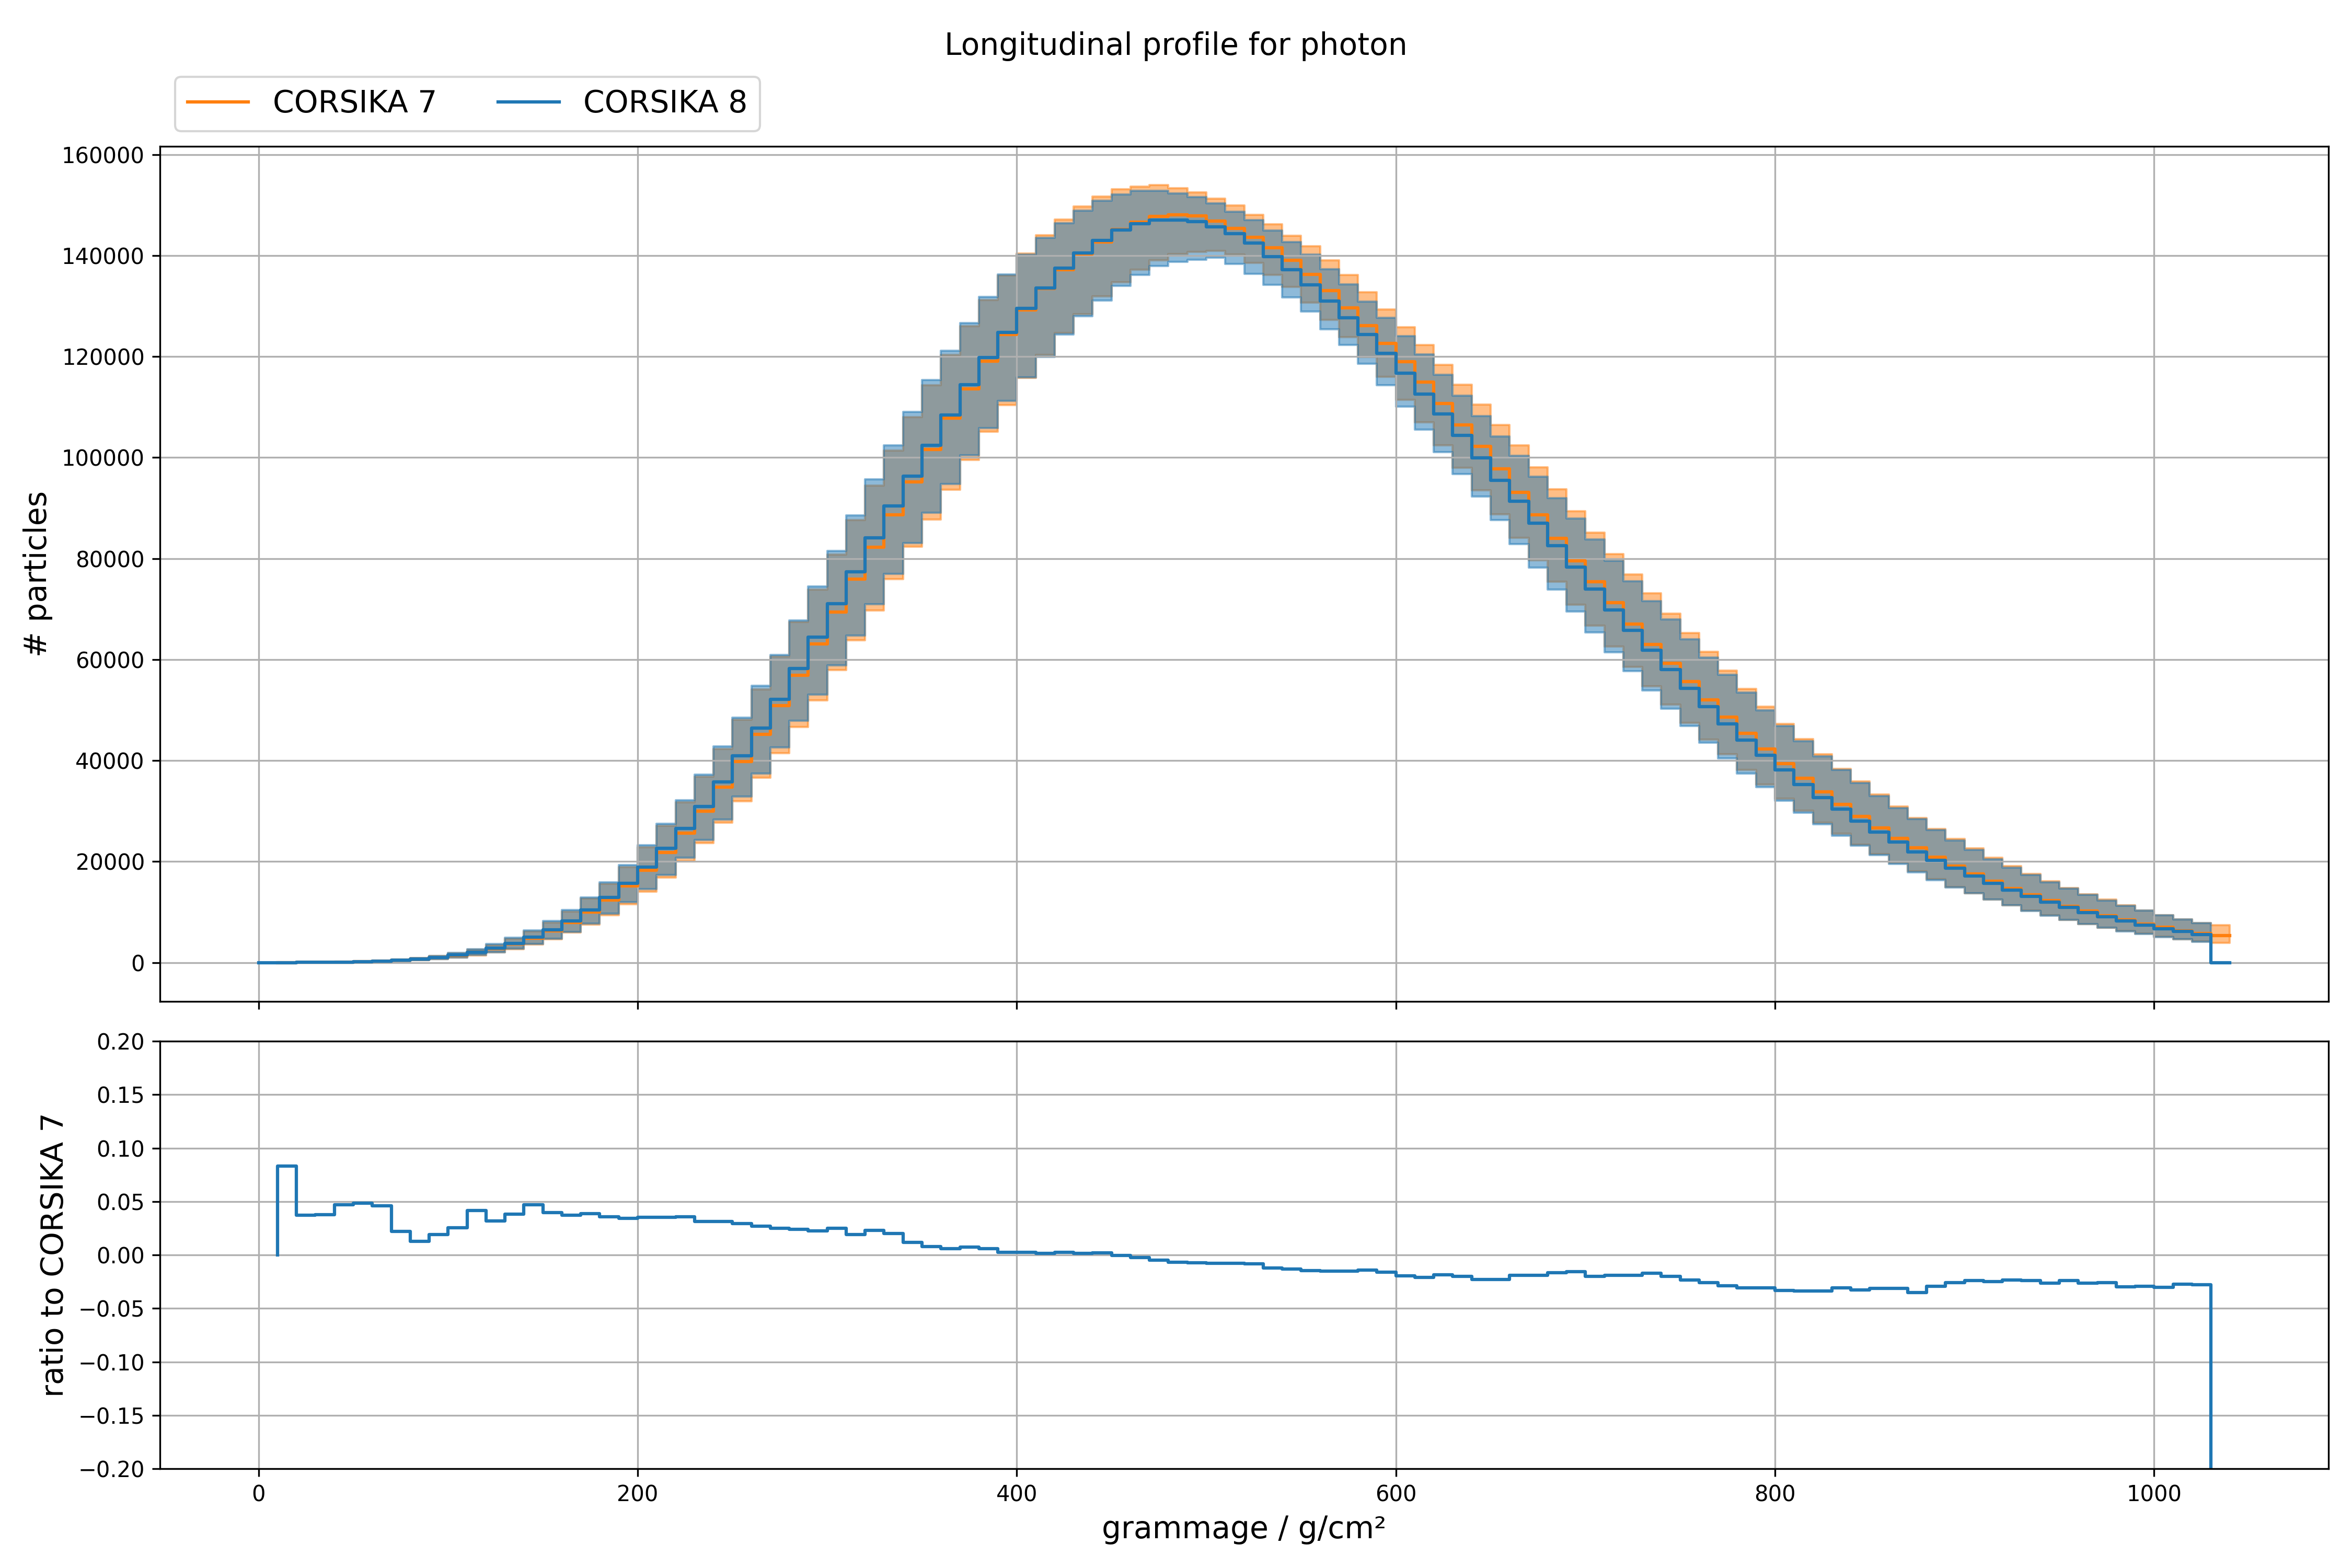
\includegraphics[width=0.95\textwidth]{plots/long_photon_2023_cherenkov.png}
                \caption{Longitudinal profile \textbf{of photons above 20 MeV} in 100 \si{\tera\electronvolt} showers, current status.}
            \end{figure}
        \end{column}
    \end{columns}
\end{frame}


\begin{frame}
  \textbf{Influence on lateral profiles}
  \vspace{5mm}

      \begin{columns}[onlytextwidth]
        \begin{column}{0.45\textwidth}
            \begin{itemize}
              \item With the fix of \texttt{Cascade}, multiple scattering is now (correctly) taken into account
              \item So far, we had always used the \texttt{Highland} parametrization of multiple scattering
              \begin{itemize}
                \item[$\rightarrow$] \texttt{Highland} is a Gaussian approximation of the complete \texttt{Molière} parametrization of multiple scattering
                \item[$\rightarrow$] The \texttt{Highland} parametrization is faster to evaluate, but neglects outliers
                \item[$\rightarrow$] Most recent release of PROPOSAL includes a parametrization of \texttt{Molière} scattering with improved performance (\texttt{MolièreInterpol})
              \end{itemize}
            \end{itemize}
        \end{column}
        \begin{column}{0.55\textwidth}
            \begin{figure}
                \centering
                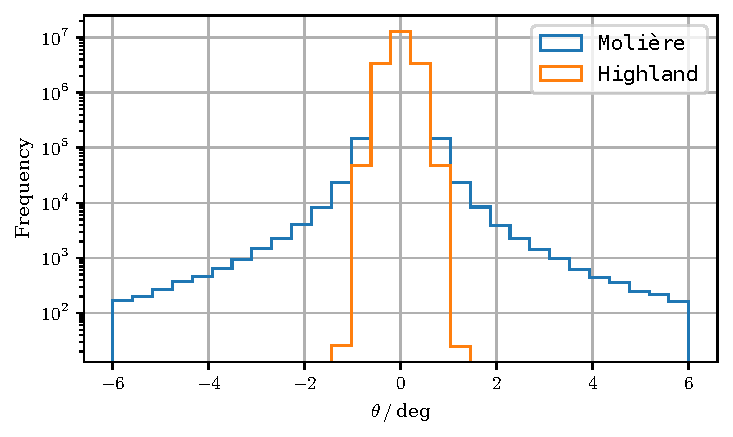
\includegraphics[width=0.95\textwidth]{plots/scattering_comparison.pdf}
                \caption{Exemplarily: Sampled scattering angles for an electron in air during a continuous step from $E_\text{i} = \SI{1}{\giga\electronvolt}$ to $E_\text{f} = \SI{0.9}{\giga\electronvolt}$, corresponding to a grammage of $X \approx \SI{3.5}{\gram\per\square\centi\meter}$.}
            \end{figure}
        \end{column}
    \end{columns}

\end{frame}


\begin{frame}
  \textbf{Influence on lateral profiles}
  \vspace{5mm}

      \begin{columns}[onlytextwidth]
        \begin{column}{0.4\textwidth}
            \begin{itemize}
              \item Lateral profiles with a better agreement (within $\SI{5}{\percent}$ for most bins)
              \item Remaining discrepancies for bins very close and very far from shower axis
            \end{itemize}
        \end{column}
        \begin{column}{0.6\textwidth}
            \begin{figure}
                \centering
                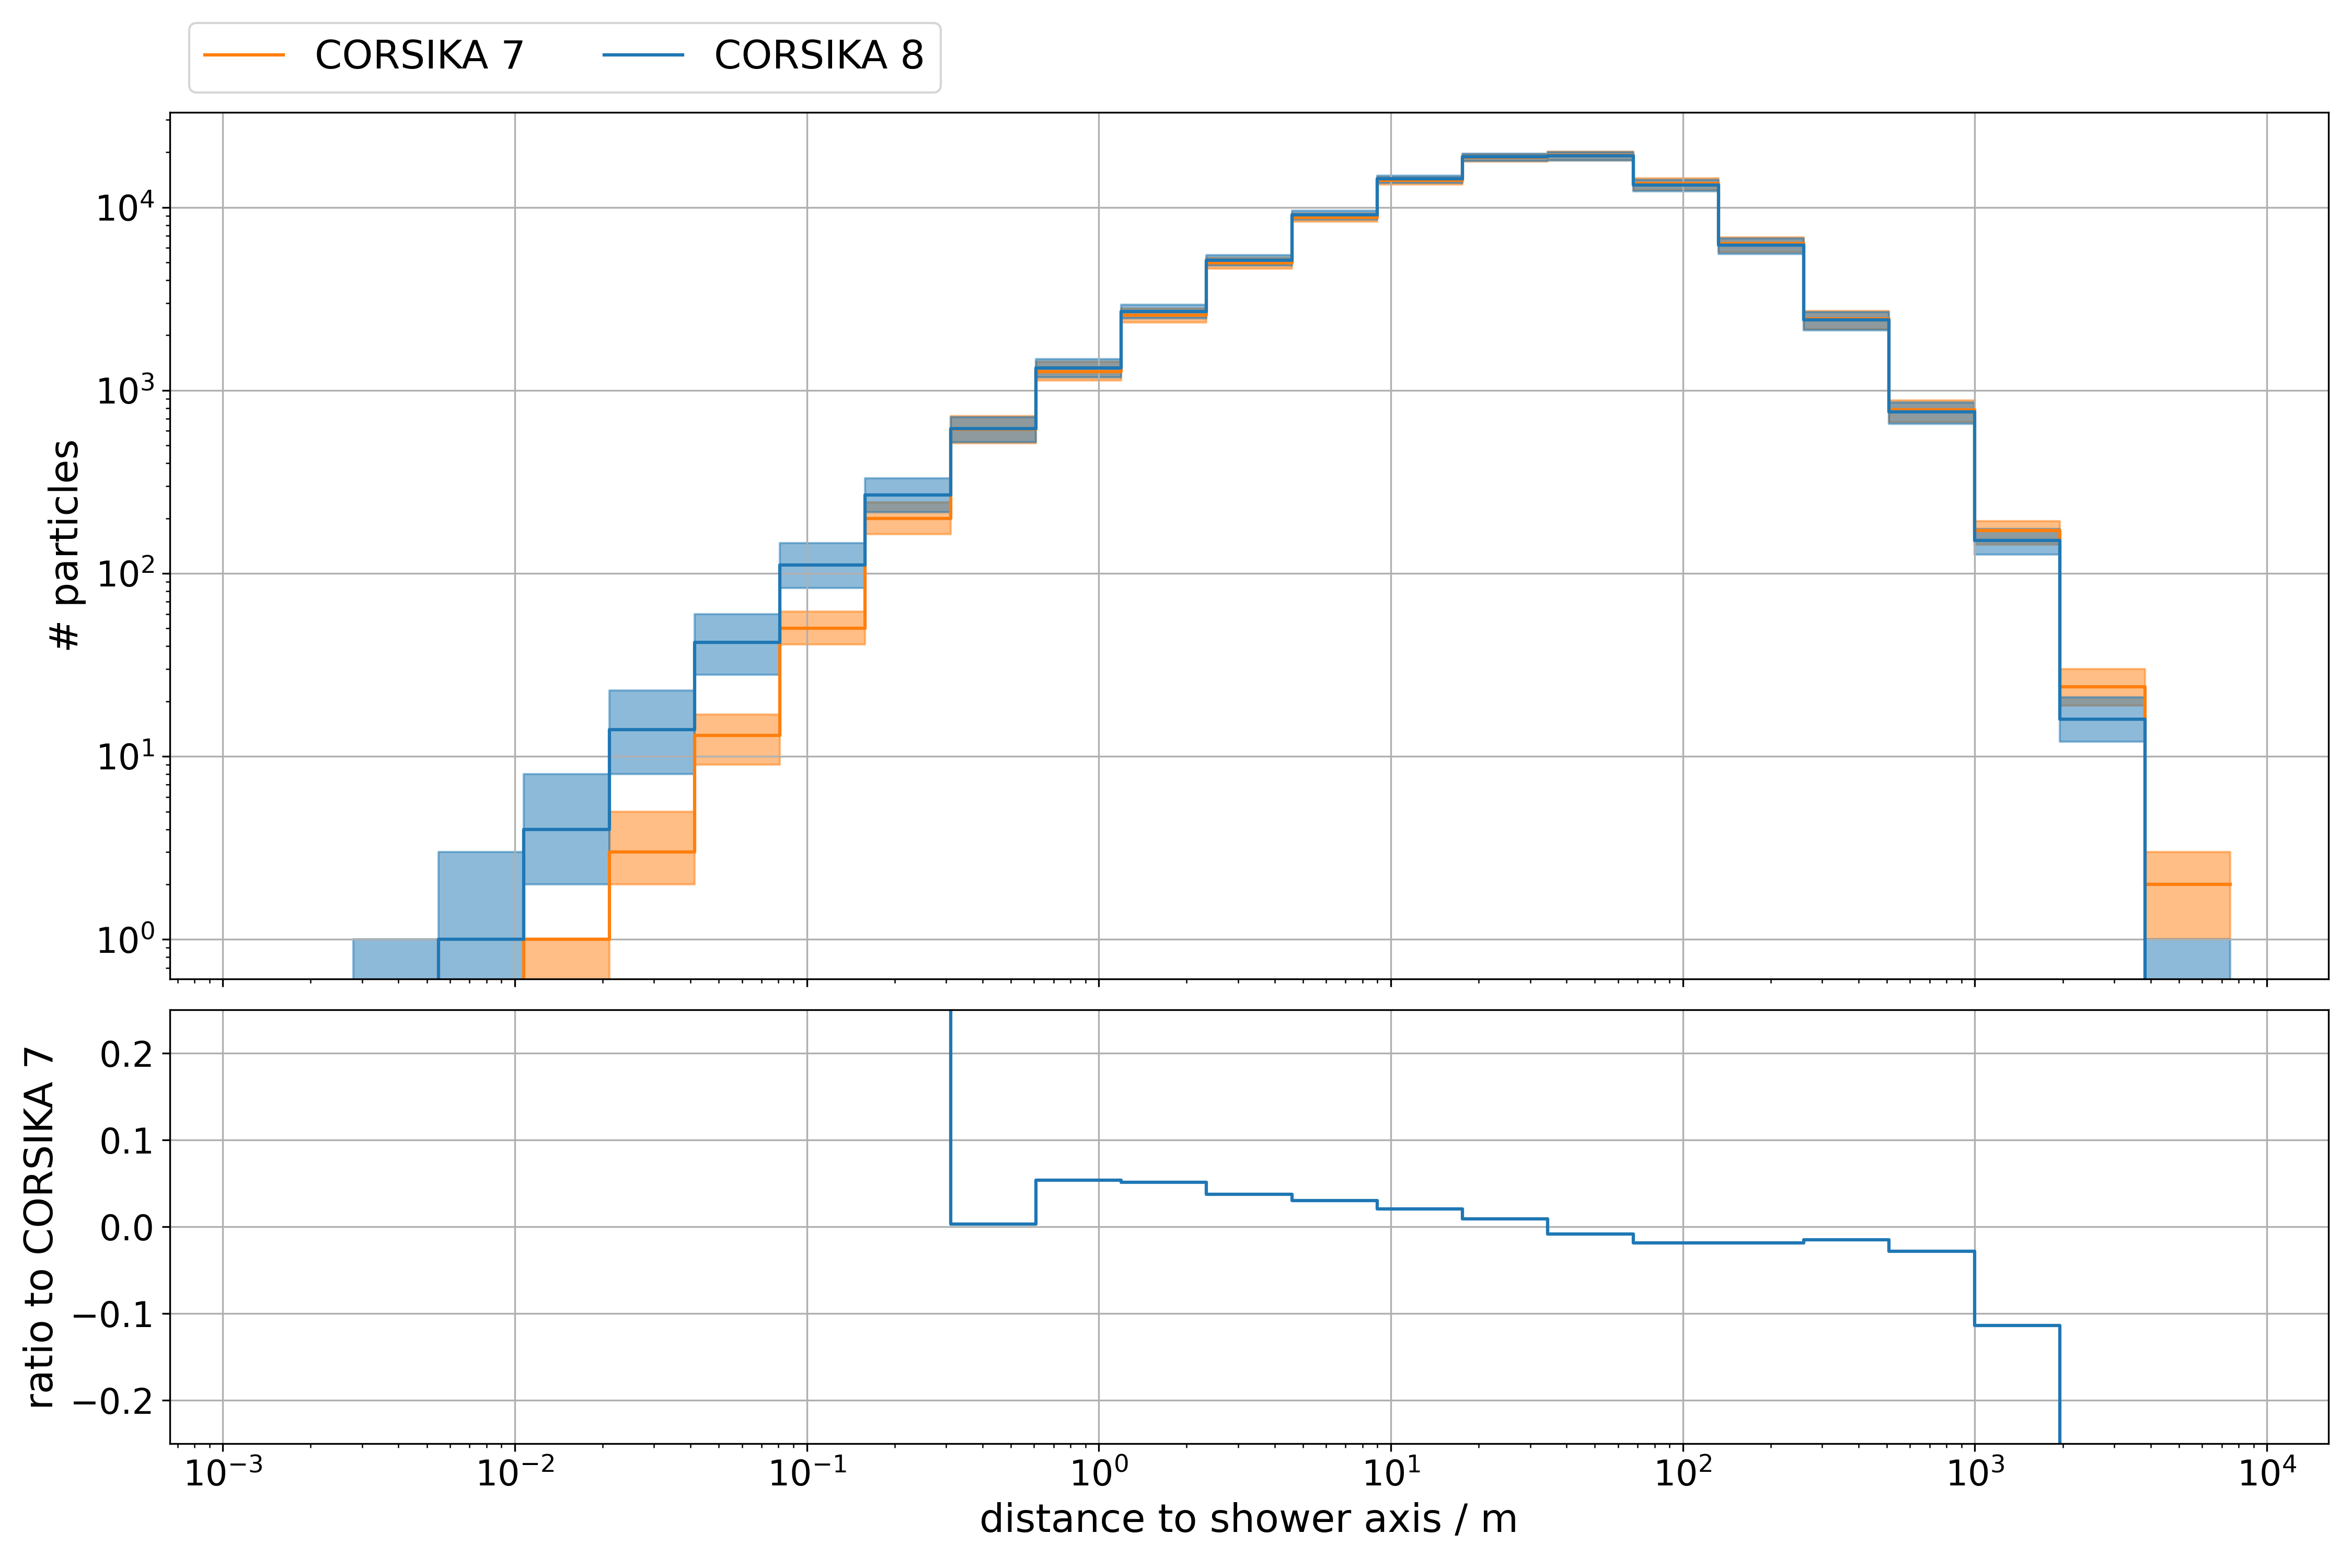
\includegraphics[width=0.95\textwidth]{plots/lateral_Charged_r_2023.png}
                \caption{Lateral profile of charged particles for 100 \si{\tera\electronvolt} showers at $X_\text{max}$, current status.}
            \end{figure}
        \end{column}
    \end{columns}

\end{frame}


\begin{frame}

\textbf{Looking back at the 2022 workshop - Which problems within the EM component did we identify?}
\vspace{5mm}
      \begin{itemize}
        \item CORSIKA~8 produce too many charged leptons (compared to CORSIKA~7)
        \begin{itemize}
          \item[$\rightarrow$] (\emoji{check-mark}) Fixed, but remaining issue for low-energy photons
        \end{itemize}
        \item CORSIKA~8 showers tend to develop earlier
        \begin{itemize}
          \item[$\rightarrow$] \emoji{x} Issue still existing
        \end{itemize}
        \item The charge excess within CORSIKA~8 is higher
        \begin{itemize}
          \item[$\rightarrow$] \emoji{check-mark} Fixed
        \end{itemize}
        \item Lateral profiles don't agree, CORSIKA~8 particles are shifted towards the shower axis
        \begin{itemize}
          \item[$\rightarrow$] (\emoji{check-mark}) Improved, but still not perfect for outliers
        \end{itemize}
      \end{itemize}

      \vspace{10mm}
      \centering
      \textbf{Big steps towards the right direction!}

\end{frame}


\begin{frame}[plain,c,noframenumbering]
  \begin{center}
    \Huge New features
  \end{center}
\end{frame}

\section{New features}


\begin{frame}

\textbf{Photoeffect}

    \begin{columns}[onlytextwidth]
        \begin{column}{0.45\textwidth}
            \begin{itemize}
              \item Implementation of an approximate treatment of the photoeffect
              \item This allows us to simulate the EM component to energies of \SI{0.5}{\mega\electronvolt} and lower
              \begin{itemize}
                \item[$\rightarrow$] Important for radio simulations
              \end{itemize}
            \end{itemize}
        \end{column}
        \begin{column}{0.55\textwidth}
            \begin{figure}
                \centering
                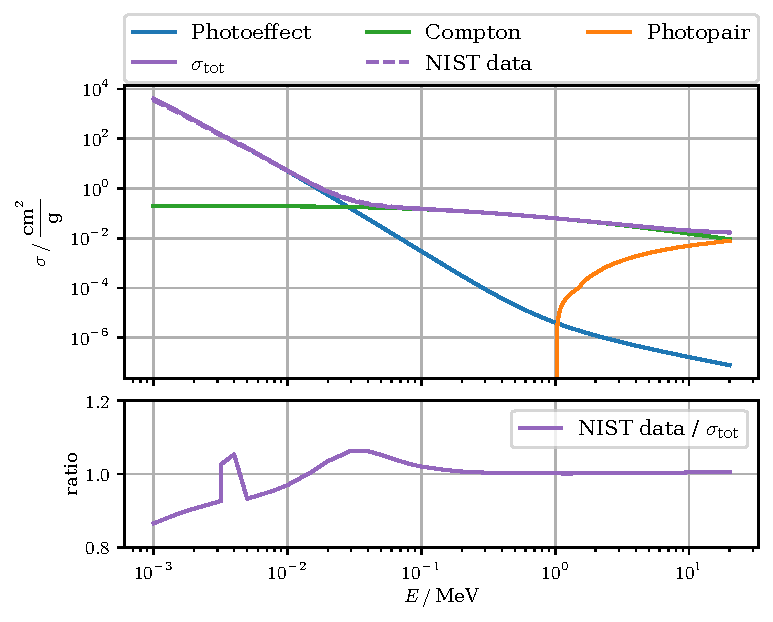
\includegraphics[width=0.95\textwidth]{plots/photoeffect_nist.pdf}
                \caption{Photon cross sections in air, compared to tables from the NIST Standard Reference Database.}
            \end{figure}
        \end{column}
    \end{columns}
\end{frame}



\begin{frame}

\textbf{LPM effect}

    \begin{columns}[onlytextwidth]
        \begin{column}{0.45\textwidth}
            \begin{itemize}
              \item The LPM effect is a suppression of bremsstrahlung and pair production
              \begin{itemize}
                \item[$\rightarrow$] Relevant for very-high energy air showers (above \SI{e18}{\electronvolt} for EM showers, above \SI{e20}{\electronvolt} for hadronic showers\footnotemark) or for dense media
              \end{itemize}
              \item Implemented as a rejection sampling for stochastic interactions
              \begin{itemize}
                \item[$\rightarrow$] No treatment for the change of continuous energy losses due to LPM implemented yet (discussion about this see \href{https://indico.scc.kit.edu/event/2580/contributions/9629/attachments/4716/7107/lpm_effect.pdf}{here})
              \end{itemize}
            \end{itemize}
        \end{column}
        \begin{column}{0.55\textwidth}
            \begin{figure}
                \centering
                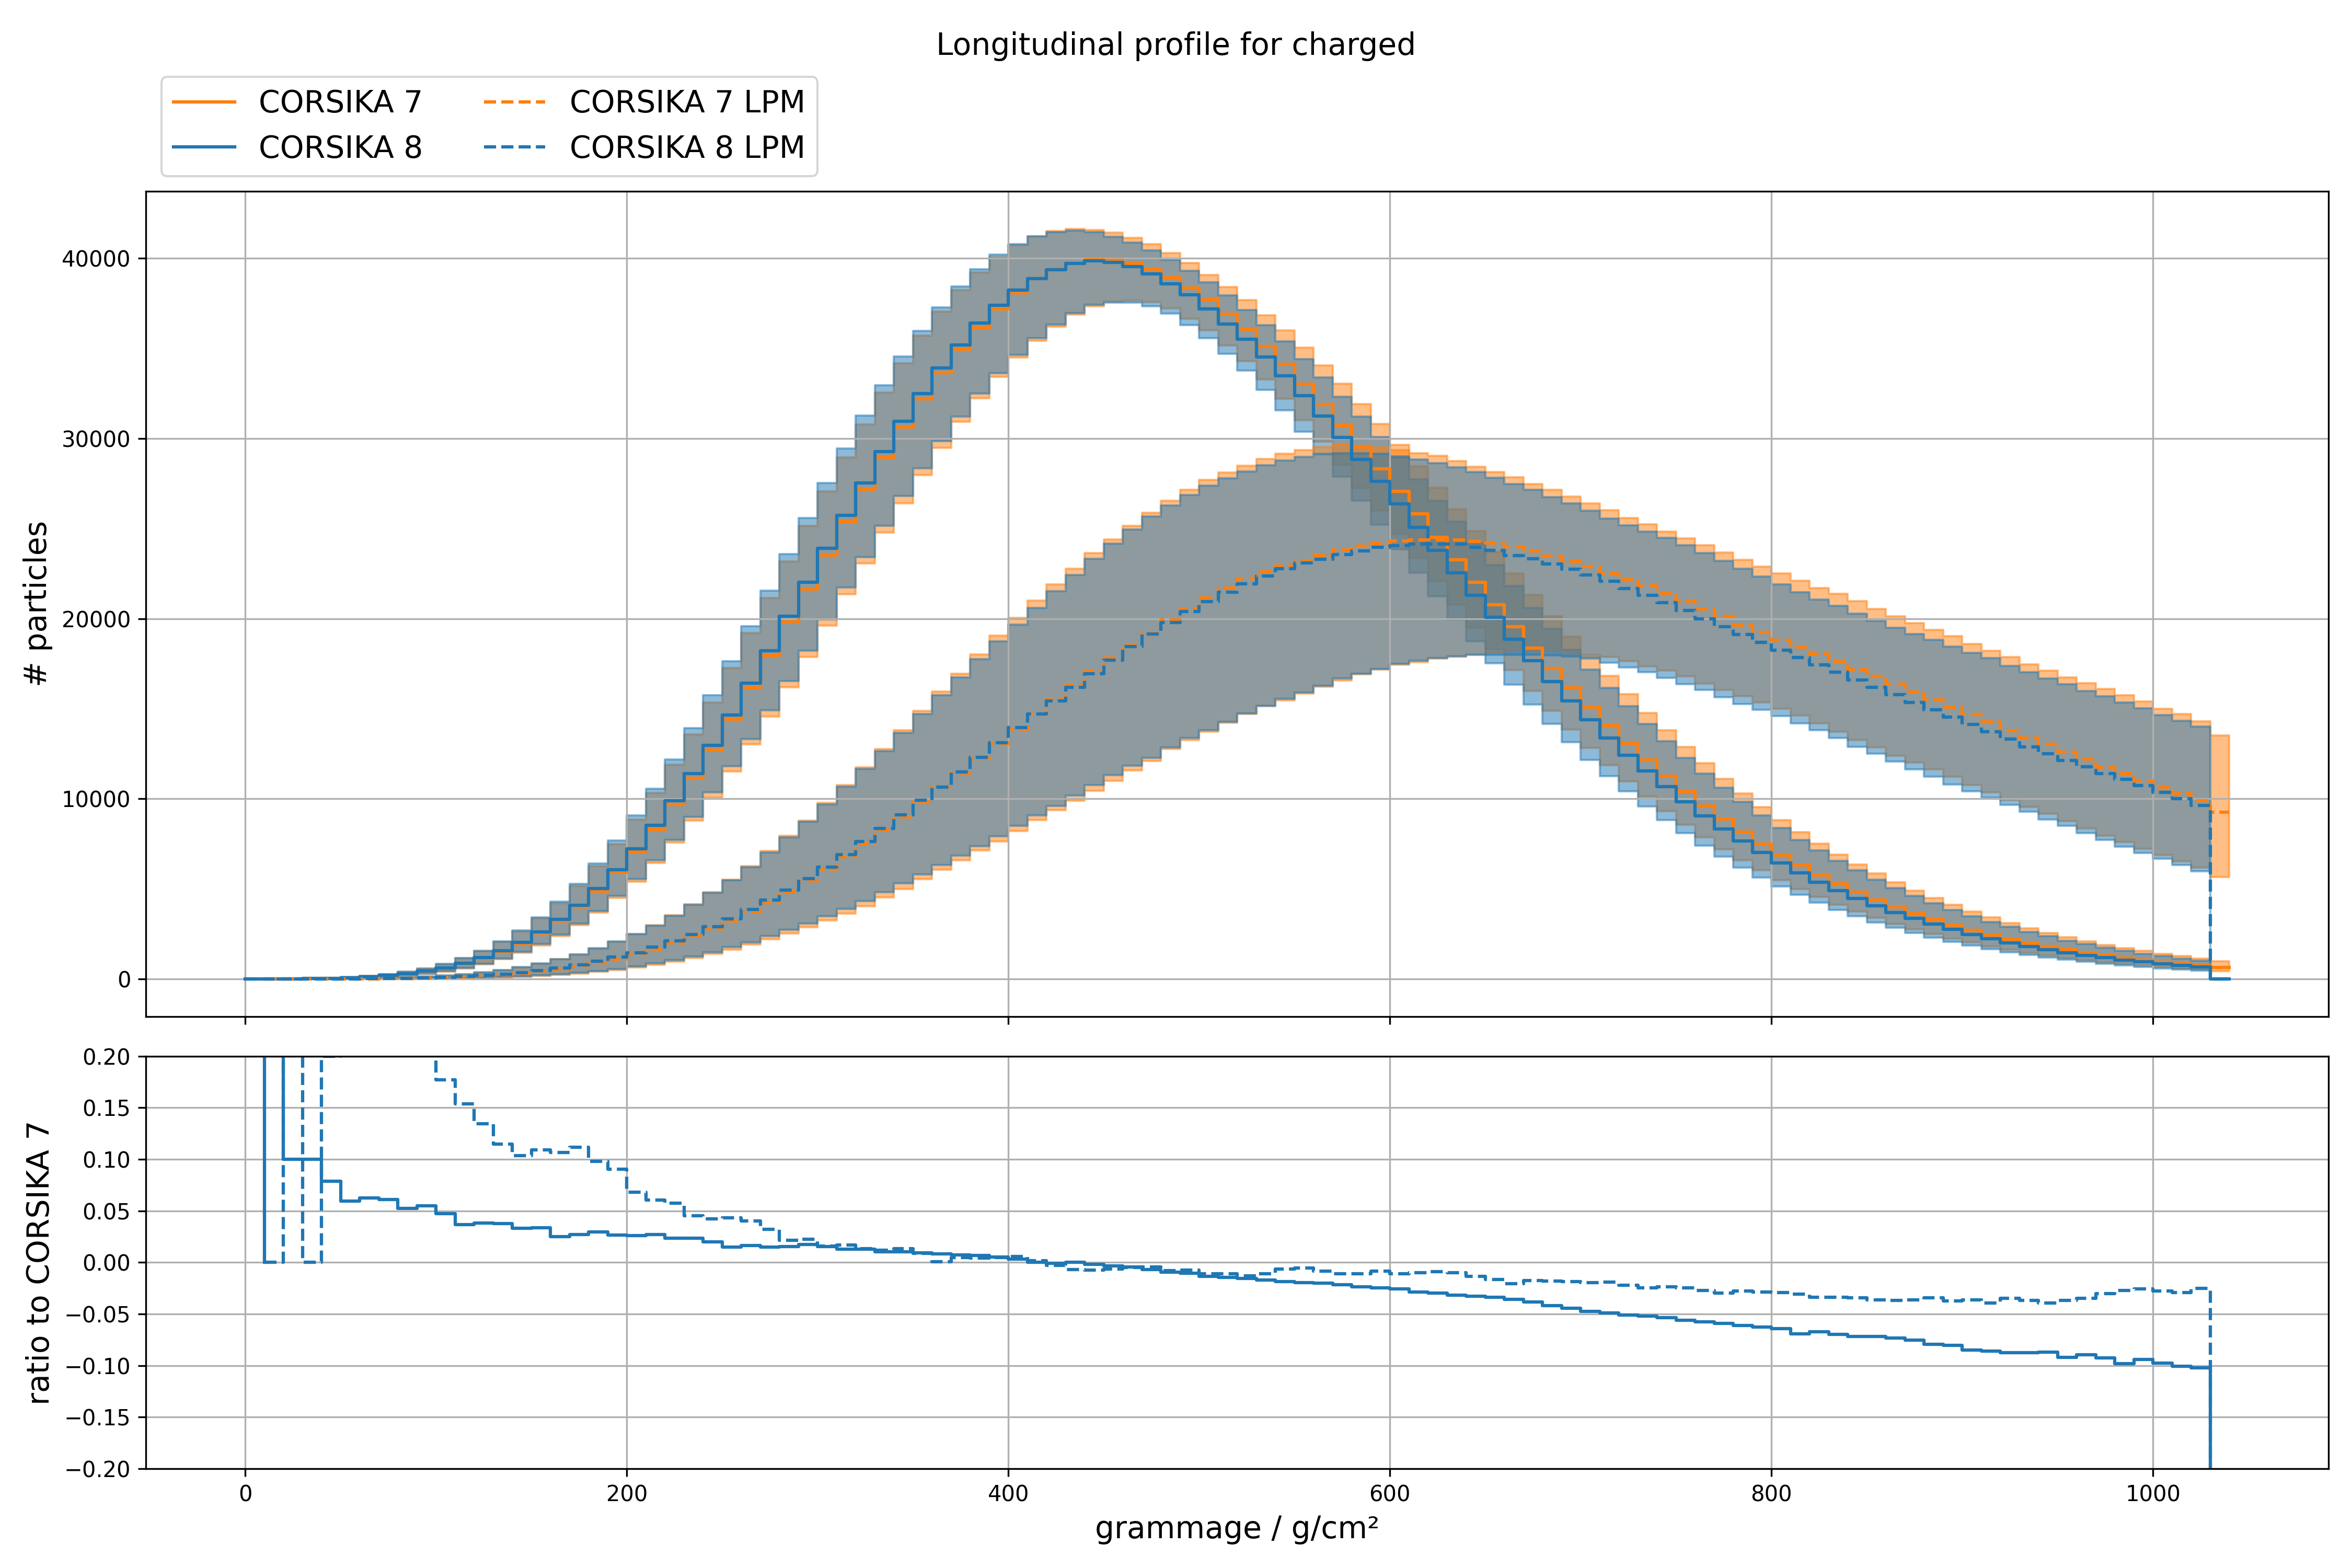
\includegraphics[width=0.95\textwidth]{plots/long_charged_LPM.png}
                \caption{Longitudinal profile for \SI{e20}{\electronvolt} showers with and without the LPM effect (simulated down to \SI{100}{\tera\electronvolt})}
            \end{figure}
        \end{column}
    \end{columns}
    \footnotetext[1]{Knapp et al., Astroparticle Physics 19.1 (2003), pp. 77–99}
\end{frame}



\begin{frame}
\textbf{Hadronic interactions in EM showers}

    \begin{itemize}
      \item Photons and charged particles can (in rare cases) interact hadronically
      \begin{itemize}
        \item[$\rightarrow$] Source of hadrons and muons from the EM component
      \end{itemize}
      \item We have an interface to SIBYLL (high-energy) and SOPHIA (low-energy) now
      \begin{itemize}
        \item[$\rightarrow$] We pass the hadronic interaction as a $\rho_0$ to the hadronic model to produce the secondary particles
      \end{itemize}
      \item In the 2022 workshop, preliminary results showed that we have less hadrons and muons compared to CORSIKA~7
      \begin{itemize}
        \item[$\rightarrow$] Back then, we only had the interface to SIBYLL
      \end{itemize}
    \end{itemize}

\end{frame}


\begin{frame}
\textbf{Hadronic interactions in EM showers}

  \begin{itemize}
    \item Now, there are significantly more muons and hadrons within our EM showers
    \item Since we are using a different approach compared to CORSIKA~7, different results are expected
    \begin{itemize}
      \item[$\rightarrow$] Requires more investigation
    \end{itemize}
  \end{itemize}

  \begin{figure}[!htb]
    \minipage{0.5\textwidth}
      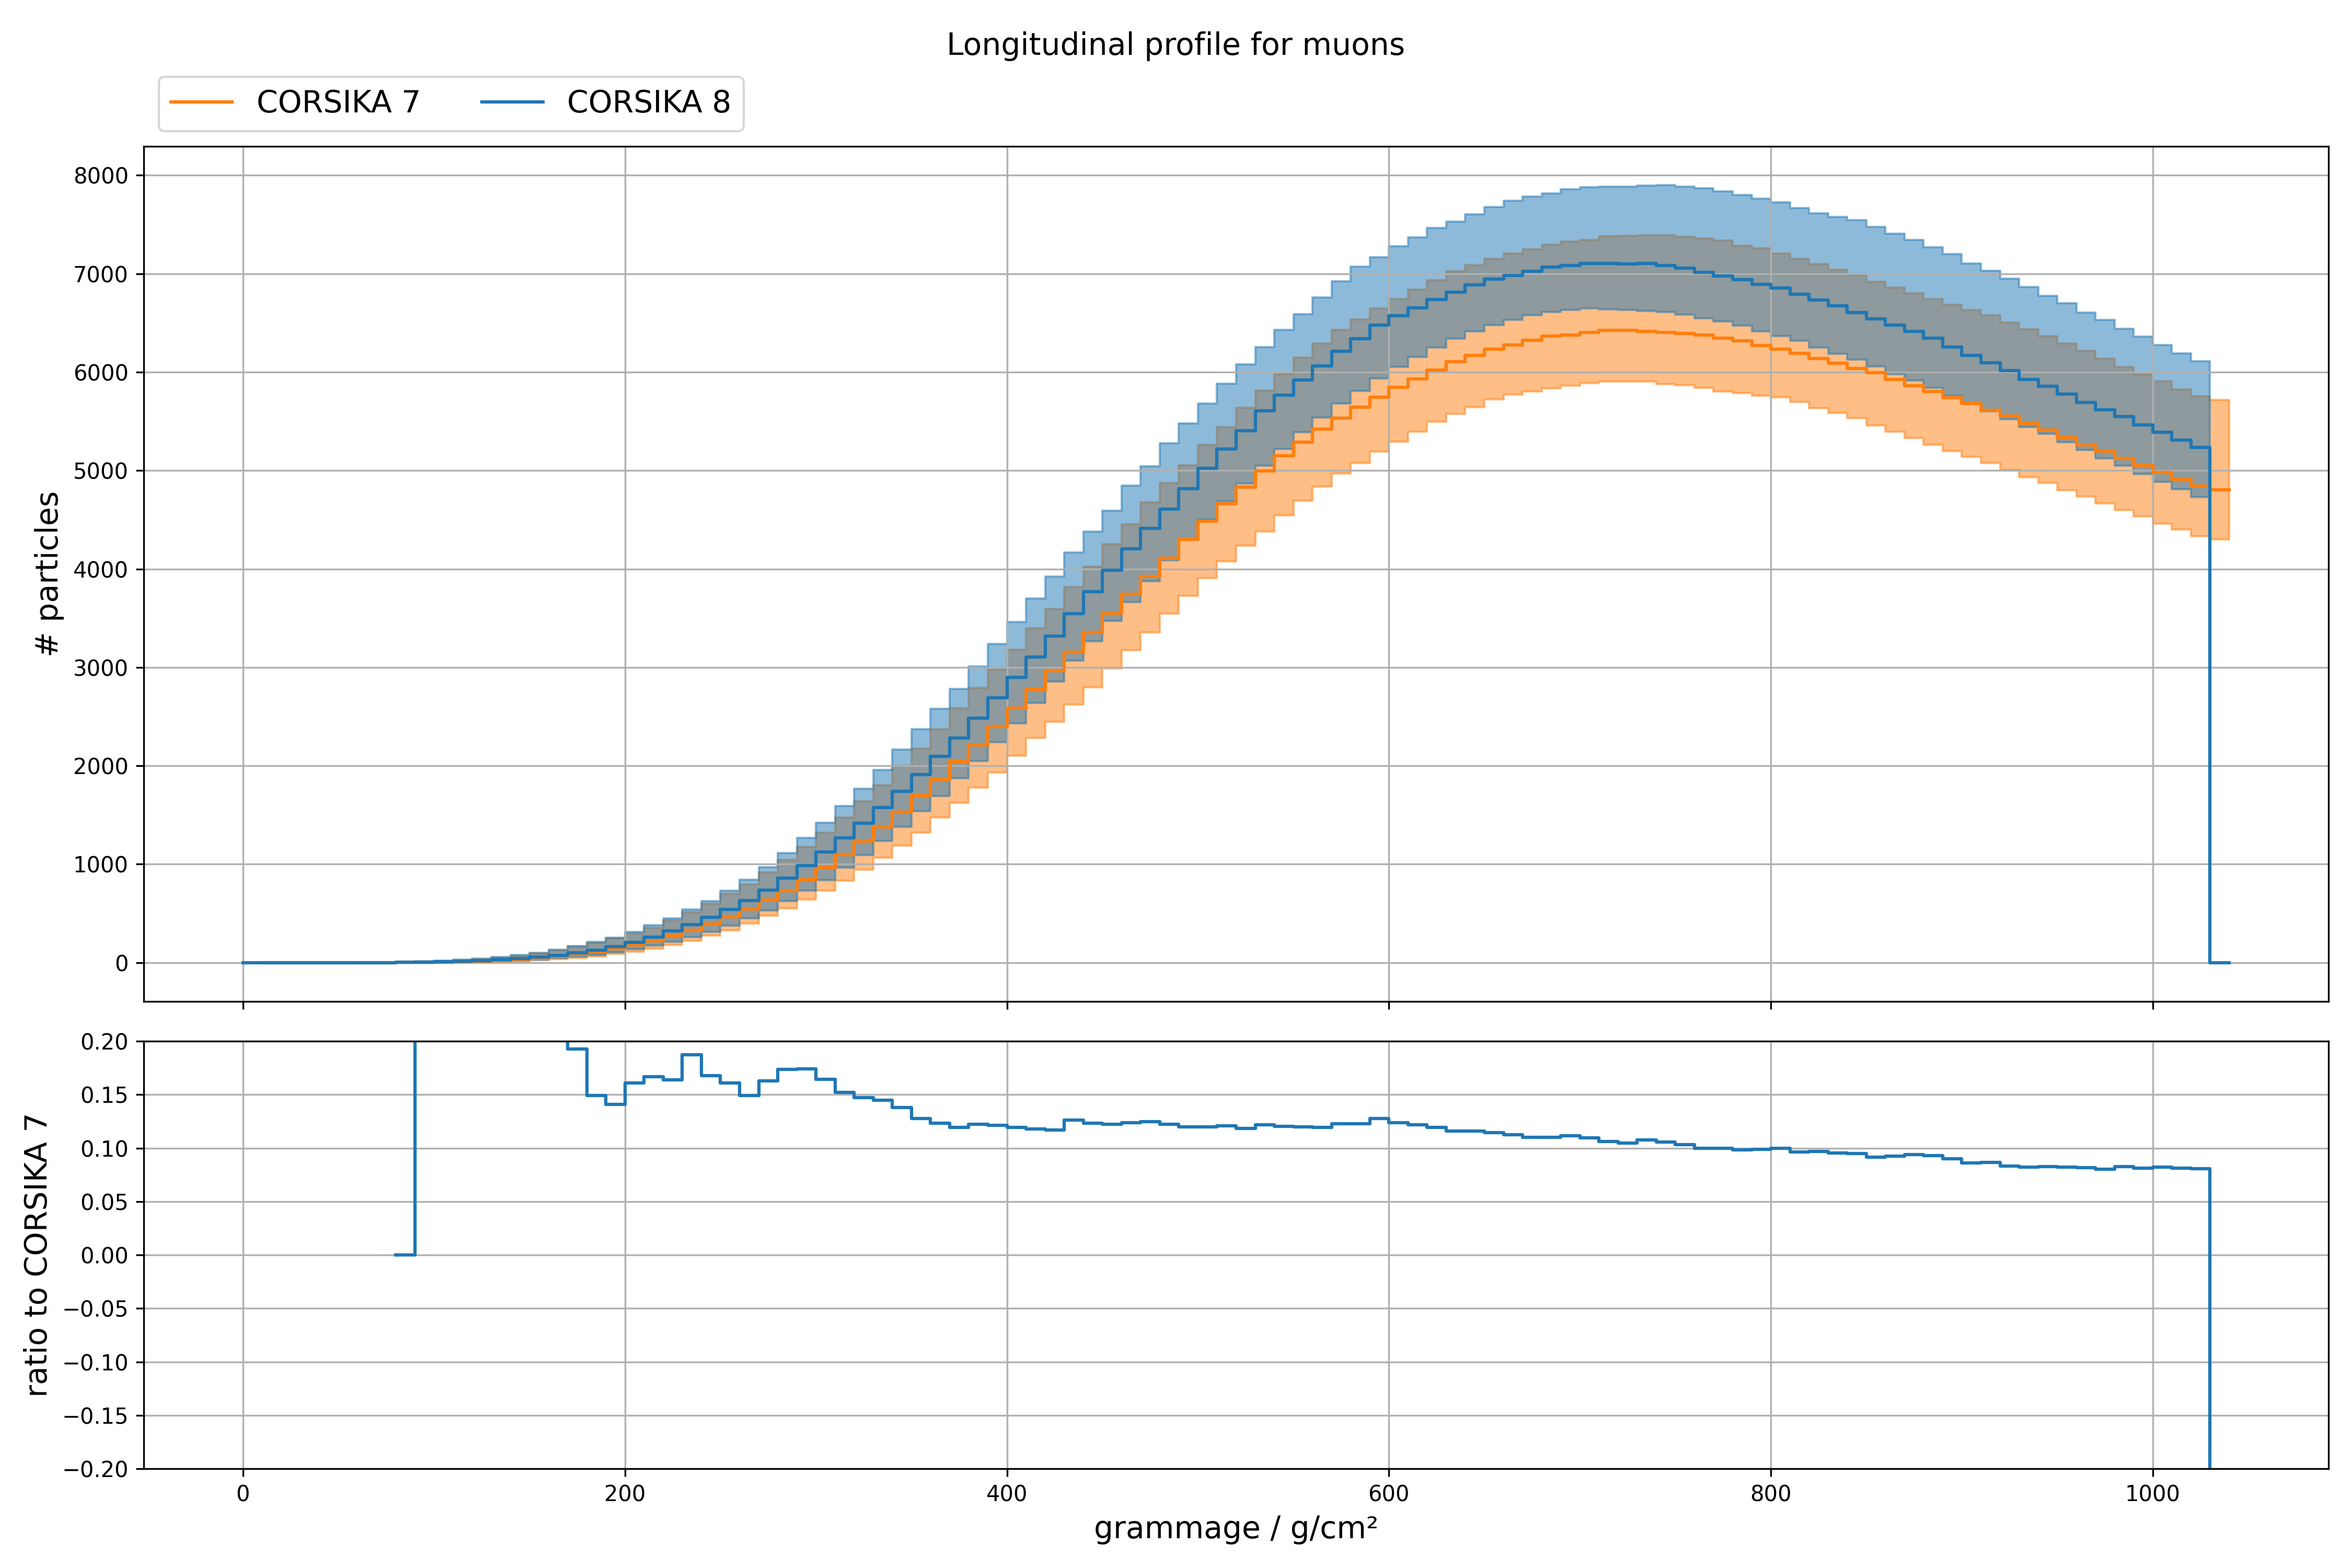
\includegraphics[width=0.95\linewidth]{plots/long_muons.png}
      \caption*{Muon distribution in 10 PeV $e^-$ showers (down to 0.5 GeV)}
    \endminipage%\hspace{3em}
    \minipage{0.5\textwidth}
      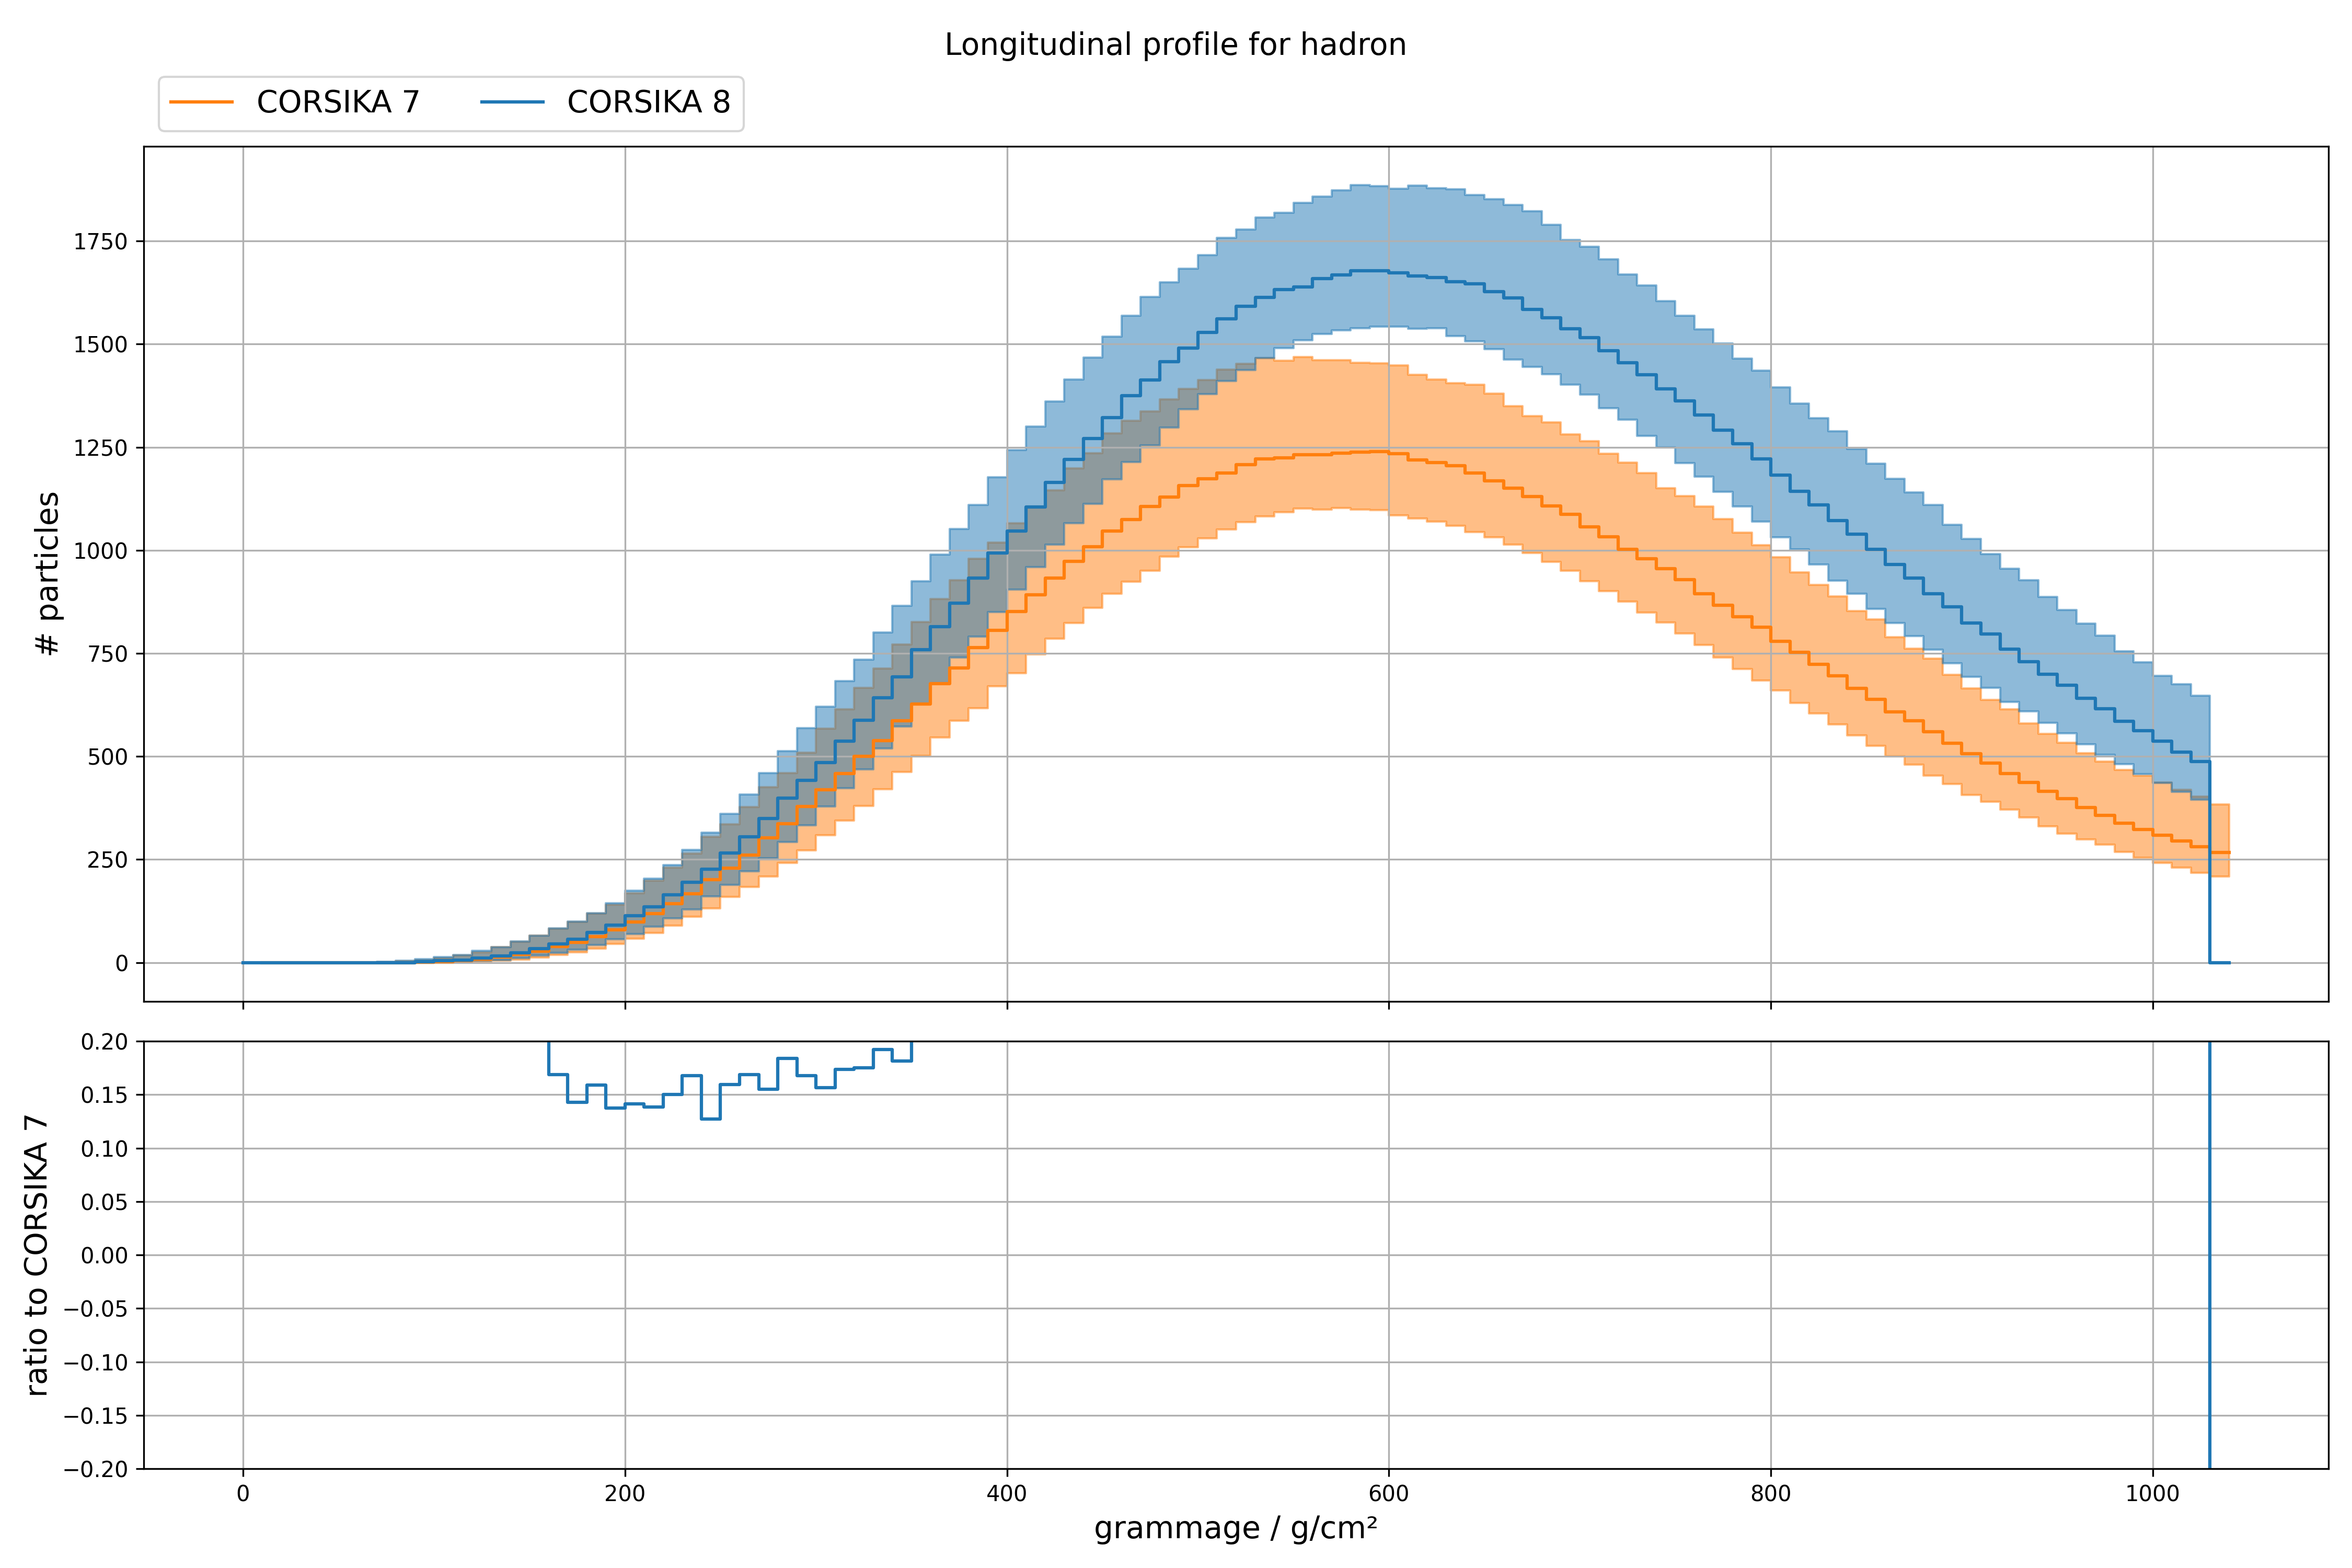
\includegraphics[width=0.95\linewidth]{plots/long_hadron.png}
      \caption*{Hadron distribution in 10 PeV $e^-$ showers (down to 0.5 GeV)}
    \endminipage
  \end{figure}
  \vspace{-0.3cm}
\end{frame}

\begin{frame}[plain,c,noframenumbering]
  \begin{center}
    \Huge Open issues, questions, and future developments
  \end{center}
\end{frame}

\section{Open issues, questions, and future developments}


\begin{frame}[c]

    \textbf{Short interlude: Concept of PROPOSAL}

    \begin{columns}[onlytextwidth]

      \begin{column}{0.5\textwidth}
        \begin{itemize}
            \item How to calculate the mean free path $\lambda \propto \sigma^{-1}$ of a particle?
            \item Naive idea: Take total cross section $\sigma = \int_{v_\text{min}}^{v_\text{max}} \frac{\symup{d}\sigma}{\symup{d}v}\, \symup{dv}$, where $v$ is the relative energy loss of a particle in a single interaction
            \begin{itemize}
                \item[$\rightarrow$] First problem: Differential cross section diverges for $v \rightarrow 0$. Therefore, $\lambda$ approaches $0$ \emoji{zap}
                \item[$\rightarrow$] Second issue: Inefficient, because this would mean we would have to sample every single interaction individually (no matter how small $v$ is!). Or in other words: We get very small steps.
            \end{itemize}
        \end{itemize}
      \end{column}

    \begin{column}{0.5\textwidth}
      \begin{figure}
        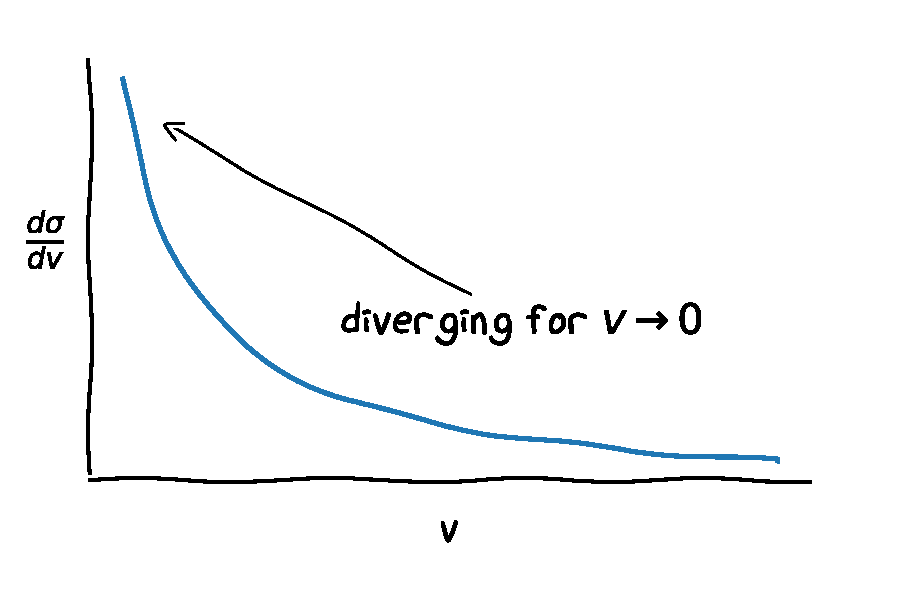
\includegraphics[width=\textwidth]{diverging_v.pdf}
      \end{figure}
    \end{column}
    \end{columns}
\end{frame}


\begin{frame}[c]
    \begin{columns}[onlytextwidth]

      \begin{column}{0.5\textwidth}
        \begin{itemize}
            \item Approach: When sampling $\lambda$, only take into account energy losses with $v > v_\text{cut}$
            \begin{itemize}
                \item[$\rightarrow$] $\sigma_\text{stoch} = \int_{v_\text{cut}}^{v_\text{max}} \frac{\symup{d}\sigma}{\symup{d}v} \, \symup{d}v$
            \end{itemize}
            \item This gives us a finite value for $\sigma_\text{stoch}$ and $\lambda_\text{stoch}$
            \item Note: This $v_\text{cut}$ can either be a relative value (e.g. \SI{1}{\percent}) or an absolute value (e.g. \SI{5}{\mega\electronvolt})
        \end{itemize}
      \end{column}

    \begin{column}{0.5\textwidth}
      \begin{figure}
        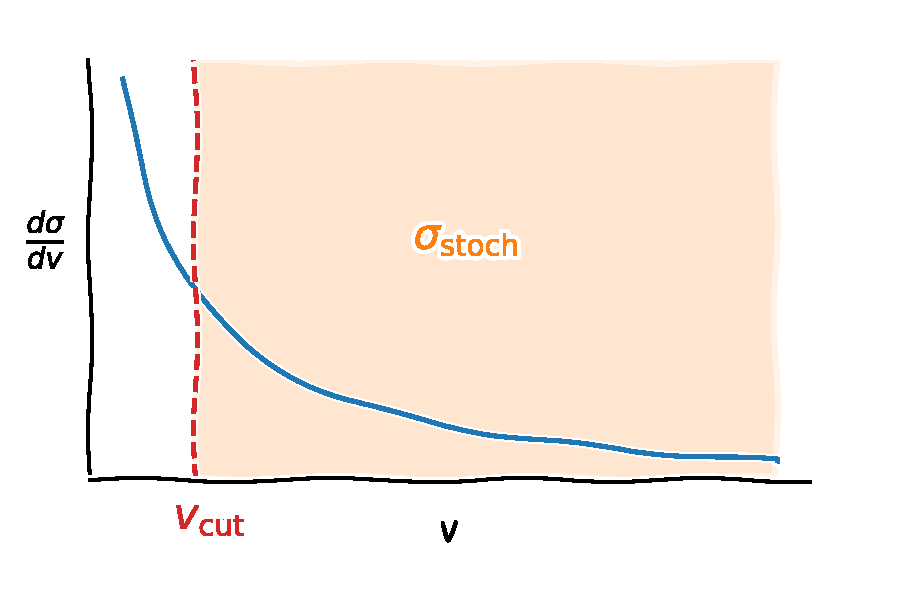
\includegraphics[width=\textwidth]{diverging_v_stoch.pdf}
      \end{figure}
    \end{column}
    \end{columns}
\end{frame}

\begin{frame}[c]
    \begin{columns}[onlytextwidth]

      \begin{column}{0.5\textwidth}
        \begin{itemize}
            \item What about the interactions with $v \leq v_\text{cut}$?
            \item We calculate an effective energy loss per distance:
            \begin{itemize}
              \item[$\rightarrow$] $\frac{\symup{d}E}{\symup{d}x} \propto E \int_{v_\text{min}}^{v_\text{cut}} v \frac{\symup{d}\sigma}{\symup{d}v} \, \symup{d}v$
            \end{itemize}
            \item Apply these continuous energy losses to propagated distance between stochastic interactions
            \item Now, all energies losses are correctly taken into account! \emoji{tada}
            \item Important question: Which value to choose for $v_\text{cut}$?
        \end{itemize}


      \end{column}

    \begin{column}{0.5\textwidth}
      \begin{figure}
        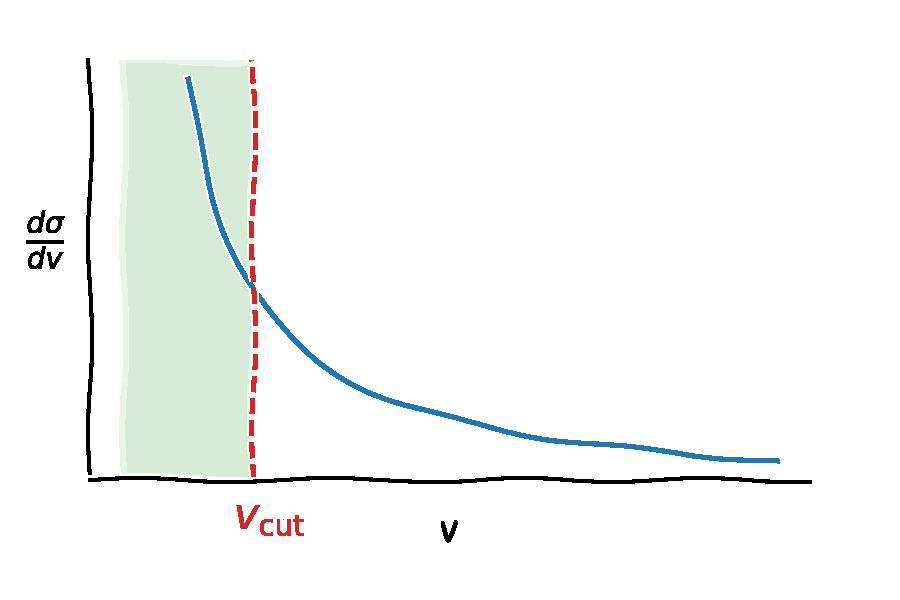
\includegraphics[width=\textwidth]{diverging_v_cont.pdf}
      \end{figure}
    \end{column}
    \end{columns}
\end{frame}


\begin{frame}

  \textbf{Usage of ParticleCut and ProductionThreshold}

  \begin{itemize}
    \item Within CORSIKA~8, there are two energy settings relevant for the EM component
    \begin{itemize}
      \item[$\rightarrow$] $\texttt{ParticleCut}$: Particles below this (total) energy are removed from the Stack
      \item[$\rightarrow$] $\texttt{ProductionThreshold}$: Only energy losses above this energy are treated stochastically. Individual energy losses below this energy are treated continuously. This is what I have just introduced as a $v_\text{cut}$.
    \end{itemize}
    \item So far, both settings have been set to an identical total energy
    \begin{itemize}
      \item[$\rightarrow$] Motivation: We don't need to individually simulate an energy loss if the produced secondary particles would be directly removed from the stack
    \end{itemize}
    \item However, recent simulations showed that there is a significant difference if one sets the \texttt{ProductionThreshold} below the \texttt{ParticleCut}
    \begin{itemize}
      \item[$\rightarrow$] This means we individually sample energy losses although we know that these particles will be directly removed from the stack
      \item[$\rightarrow$] However, this might be necessary for an accurate simulation of the shower development, since the approximation as a continuous energy loss might be inaccurate.
    \end{itemize}
  \end{itemize}
\end{frame}


\begin{frame}

  \textbf{Usage of ParticleCut and ProductionThreshold}


    \begin{columns}[onlytextwidth]
        \begin{column}{0.45\textwidth}
            \begin{itemize}
              \item Possible solutions: 
              \begin{enumerate}
                \item Set the \texttt{ProductionThreshold} to a fraction of the \texttt{ParticleCut} (e.g. \SI{1}{\percent})
                \item Introduce a relative \texttt{ProductionThreshold} in addition to the absolute one. This is intrinsically possible with PROPOSAL (called $v_\text{cut}$).
              \end{enumerate}
              \item Plot on the right shows the comparison to a simulation where the $v_\text{cut}$ has been included
              \begin{itemize}
                \item[$\rightarrow$] Much better agreement with CORSIKA~7.
              \end{itemize}
              \item Maybe a point of discussion for the working sessions
            \end{itemize}
        \end{column}
        \begin{column}{0.55\textwidth}
            \begin{figure}
                \centering
                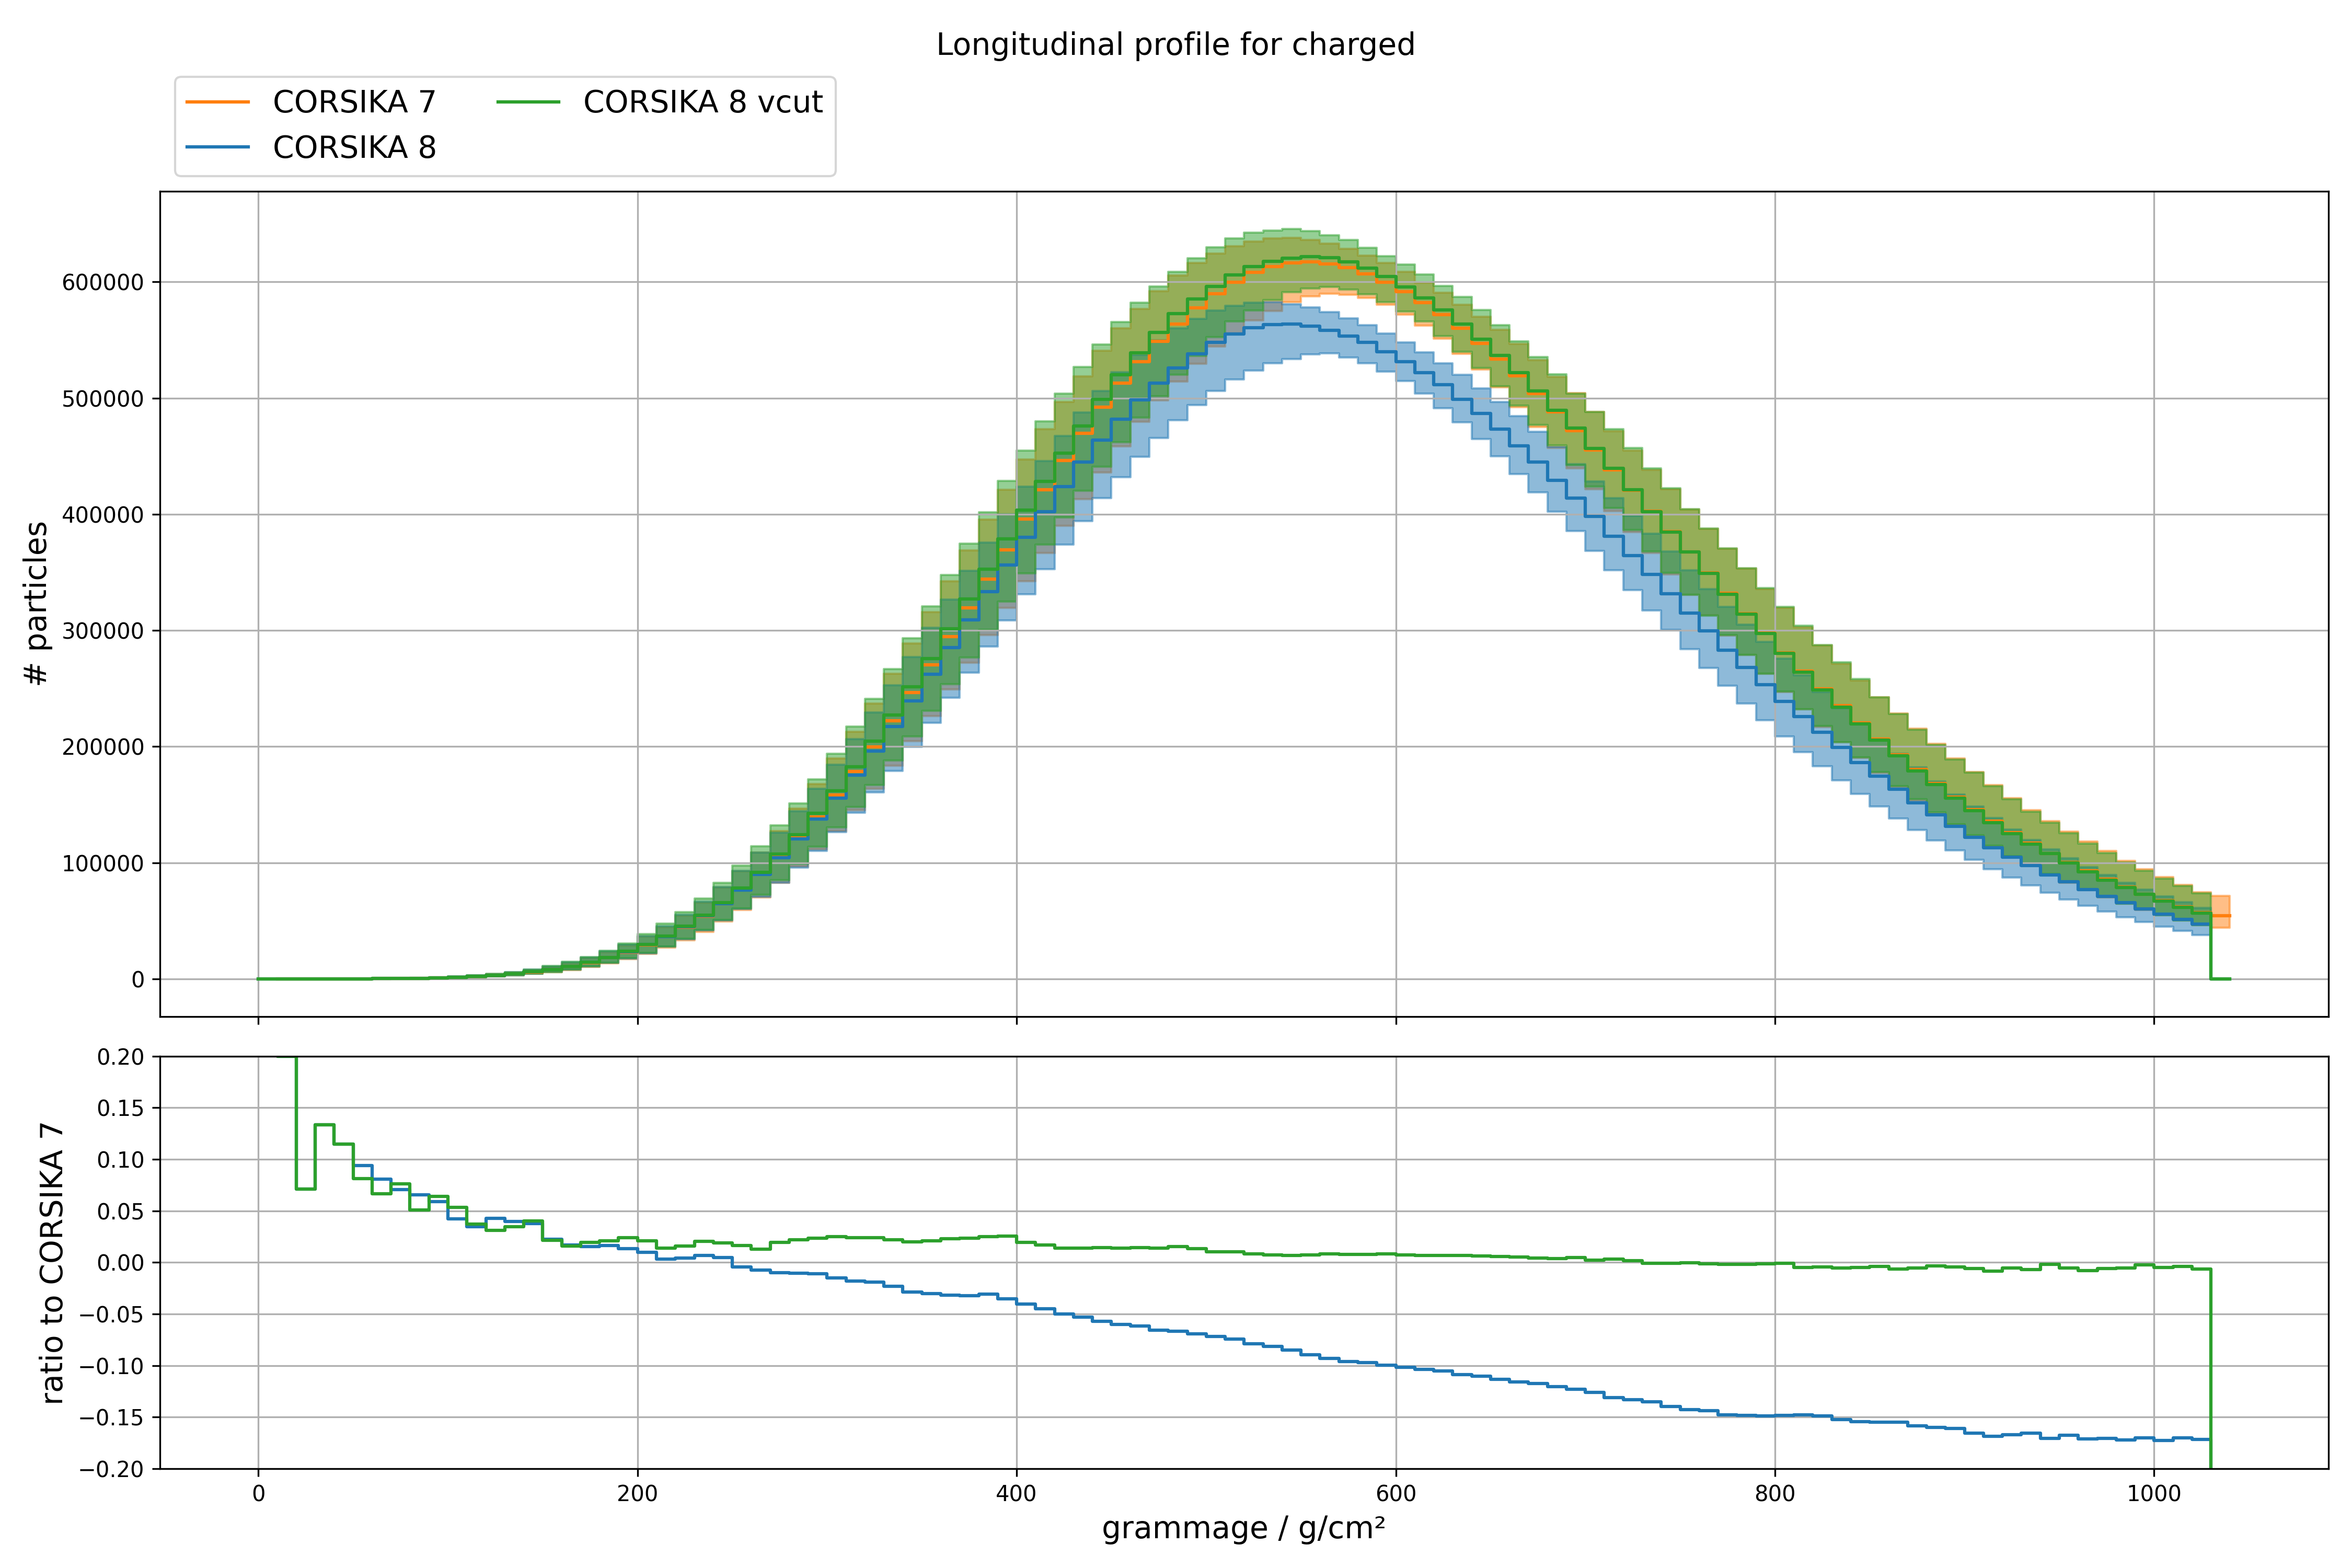
\includegraphics[width=0.95\textwidth]{plots/long_charged_vcut.png}
                \caption{Longitudinal profile of charged particles in 10 PeV $e^-$ showers (down to 0.5 GeV)}
            \end{figure}
        \end{column}
    \end{columns}
\end{frame}


\begin{frame}

  \textbf{Lateral particle development}


    \begin{columns}[onlytextwidth]
        \begin{column}{0.5\textwidth}
            \begin{itemize}
              \item Multiple scattering is working much better now
              \item However, a complete treatment of multiple scattering should include the change of direction after a continuous step and the lateral displacement of the particle
              \begin{itemize}
                \item[$\rightarrow$] Treatment is highly non-trivial, see discussion and \href{https://indico.scc.kit.edu/event/2711/contributions/10845/attachments/5244/8030/talk.pdf}{slides} of last workshop. 
                \item[$\rightarrow$] More advanced algorithmic treatment of continuous step like \emph{RandomHinge} or \emph{numerical particle propagation} as \href{https://indico.scc.kit.edu/event/2711/contributions/10924/attachments/5269/8076/propagation.pdf}{presented by Maximilian at the last workshop} 
              \end{itemize}
              \item Still not included, but important: Path length correction due to multiple scattering
            \end{itemize}
        \end{column}
        \begin{column}{0.5\textwidth}

      \centering
      \begin{figure}
        \tcbox{
         \begin{tikzpicture}[scale=1.0, every node/.style={scale=1.0}]
             \centering
             \draw [-stealth, densely dotted](0,0) -- (1.2,0) node[midway, above]{$\substack{\text{initial} \\ \text{direction}}$};
             \draw [-stealth, line width=0.4mm](1.4,0) -- (3.2,0) node[midway, above]{$\substack{\text{continuous} \\ \text{step}}$};
             \draw [-stealth, densely dotted](3.4,0) -- (4.8,0) node[midway, above]{$\substack{\text{final} \\ \text{direction}}$};
         \end{tikzpicture}
        }
      \end{figure}

      \begin{figure}
        \tcbox{
         \begin{tikzpicture}[scale=1.0, every node/.style={scale=1.0}]
             \centering
             \draw [-stealth, densely dotted](0,0) -- (1.2,0) node[midway, above]{$\substack{\text{initial} \\ \text{direction}}$};
             \draw [-stealth, line width=0.4mm](1.4,0) -- (3.2,0) node[midway, above]{$\substack{\text{continuous} \\ \text{step}}$};
             \draw [-stealth, densely dotted](3.4,0) -- (4.8,0.2) node[midway, above]{$\substack{\text{final} \\ \text{direction}}$};
         \end{tikzpicture}
        }
      \end{figure}


      \begin{figure}
      \tcbox{
         \begin{tikzpicture}[scale=1.0, every node/.style={scale=1.0}]
             \centering
             \draw [-stealth, densely dotted](0,0) -- (1.2,0) node[midway, above]{$\substack{\text{initial} \\ \text{direction}}$};
             \draw [-stealth, line width=0.4mm](1.4,0) -- (3.2,0.2) node[midway, above]{$\substack{\text{continuous} \\ \text{step}}$};
             \draw [-stealth, densely dotted](3.4,0.2) -- (4.8,0.58) node[midway, above]{$\substack{\text{final} \\ \text{direction}}$};
         \end{tikzpicture}
        }
      \end{figure}

        \end{column}
    \end{columns}
\end{frame}

\begin{frame}

  \textbf{Some other aspects...}

   \vspace{3mm}

  \emph{Open pull requests}

    \begin{itemize}
      \item \sout{LPM effect implementation} $\rightarrow$ Merged on monday!
      \item Stochastic photon propagation
      \begin{itemize}
        \item[$\rightarrow$] No continuous losses for photons anymore. Numerically more stable, less warnings, no endless loops.
      \end{itemize}
      \item Update to PROPOSAL 7.6.1
      \begin{itemize}
        \item[$\rightarrow$] Includes some vital bugfixes, e.g. for ionization losses
        \item[$\rightarrow$] \texttt{MolièreInterpol}, significant speed-up of multiple scattering
        \item[$\rightarrow$] Improved sampling methods for pairproduction ($\theta$) and tripet production ($\rho$)
      \end{itemize}
    \end{itemize}

  \emph{Points of discussion}

  \begin{itemize}
    \item Steering of the options provided by PROPOSAL
    \begin{itemize}
        \item[$\rightarrow$] PROPOSAL has a flexible structure, allowing users to adapt/change physics parametrizations
        \item[$\rightarrow$] How to combine these features with steering of CORSIKA~8?
    \end{itemize}
    \item Table creation
    \begin{itemize}
        \item[$\rightarrow$] Current solution not optimal for users
        \item[$\rightarrow$] Already had some discussions yesterday after Alexanders talk, in the coffee break, and on the train
    \end{itemize}
   \end{itemize}


\end{frame}




\begin{frame}[plain,c,noframenumbering]
  \begin{center}
    \Huge Summary
  \end{center}
\end{frame}

\section{Summary}

\begin{frame}

    \begin{itemize}
      \item A lot of issues have been fixed since the last workshop
      \item What has not been mentioned: A large amount of smaller and larger bugfixes that helped improved the stability of CORSIKA~8
      \begin{itemize}
        \item[$\rightarrow$] Less crashes and warnings due to the EM component \emoji{crossed-fingers}
      \end{itemize}
      \item All relevant physics processes are included by now
      \item Some improvements and investigations are still necessary
      \begin{itemize}
        \item[$\rightarrow$] Lateral shower development
        \item[$\rightarrow$] Hadronic interactions in EM showers
        \item[$\rightarrow$] Low-energy photons
      \end{itemize}
      \item Elephant in the room not mentioned in this talk: Need for runtime optimization \emoji{elephant}
    \end{itemize}
\end{frame}


\appendix

\begin{frame}[plain,c,noframenumbering]
  \begin{center}
    \Huge Backup
  \end{center}
\end{frame}


\begin{frame}[plain,c,noframenumbering]
  \begin{center}
    \Huge Studies of $v_\text{cut}$ settings
  \end{center}
\end{frame}


\begin{frame}
            \begin{figure}
                \centering
                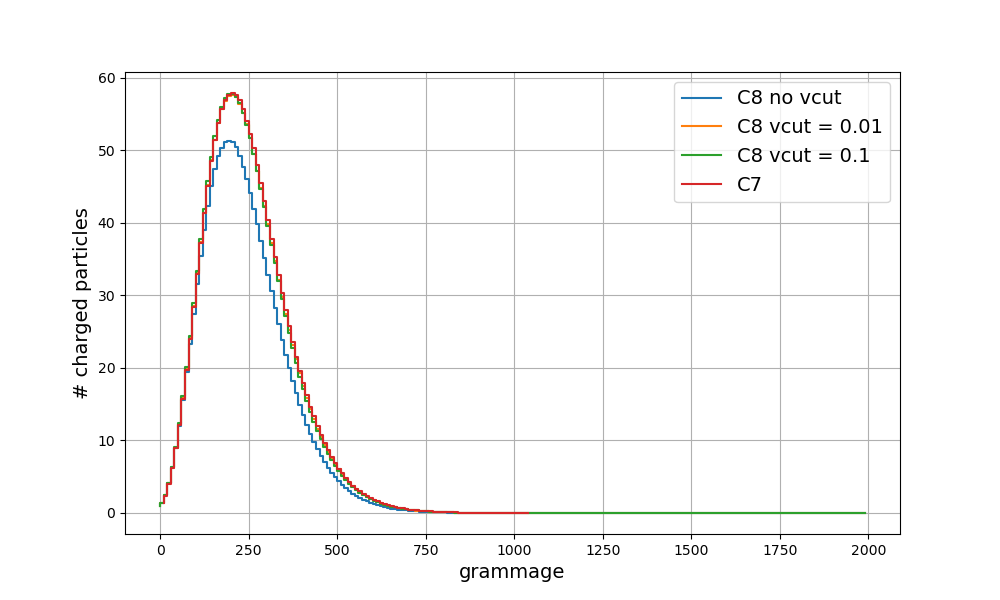
\includegraphics[width=0.75\textwidth]{plots/v_analysis_charged.png}
                \caption{Longitudinal profile of charged particles in 100 PeV $e^-$ showers, using different (or none) $v_\text{cut}$ settings.}
            \end{figure}
\end{frame}

\begin{frame}
            \begin{figure}
                \centering
                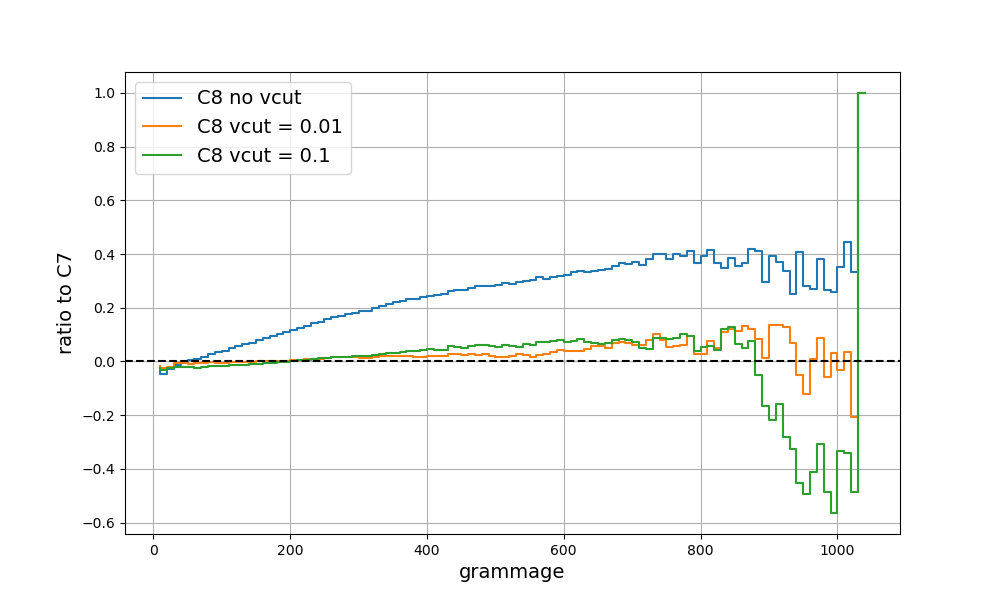
\includegraphics[width=0.75\textwidth]{plots/v_analysis_charged_ratio.png}
                \caption{Longitudinal profile of charged particles in 100 PeV $e^-$ showers, using different (or none) $v_\text{cut}$ settings.}
            \end{figure}
\end{frame}

\begin{frame}
            \begin{figure}
                \centering
                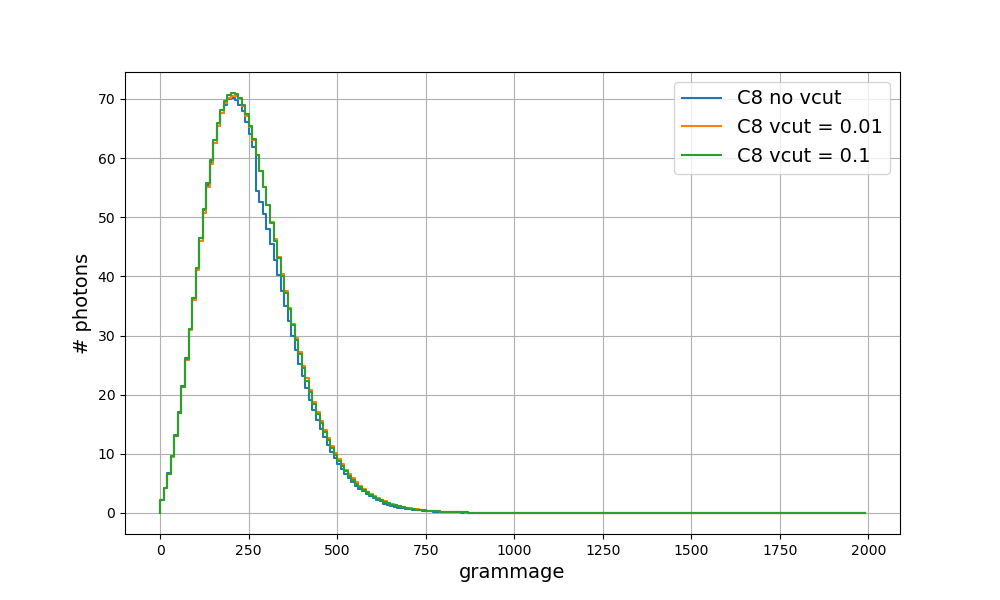
\includegraphics[width=0.75\textwidth]{plots/v_analysis_photon.png}
                \caption{Longitudinal profile of photons in 100 PeV $e^-$ showers, using different (or none) $v_\text{cut}$ settings.}
            \end{figure}
\end{frame}

\begin{frame}[plain,c,noframenumbering]
  \begin{center}
    \Huge Effects of $e_\text{cut}$ and $v_\text{cut}$
  \end{center}
\end{frame}


\begin{frame}
            \begin{figure}
                \centering
                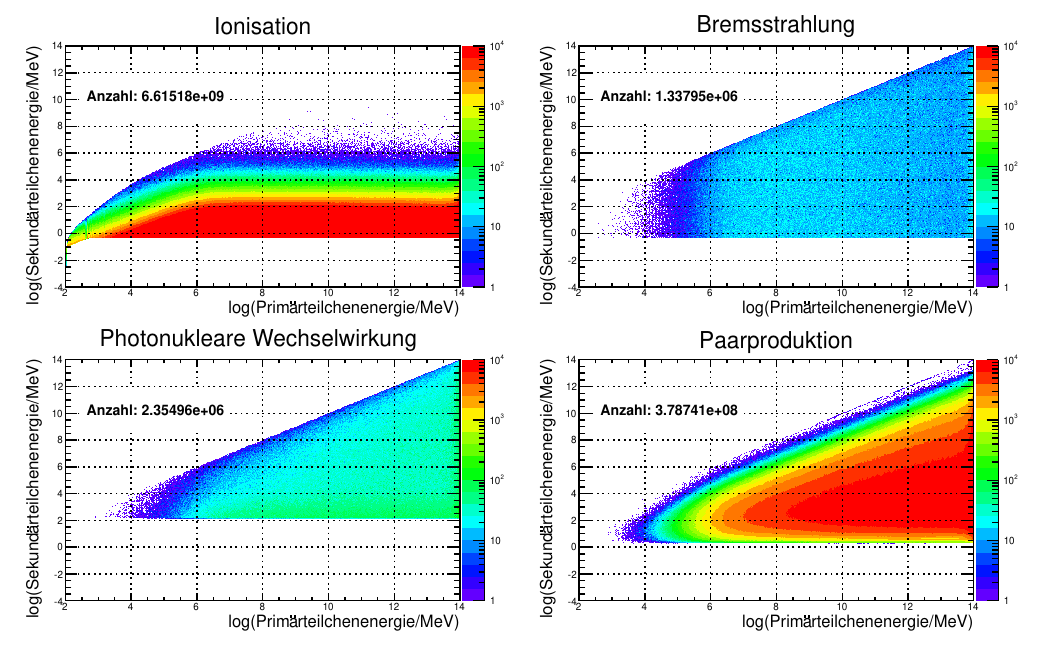
\includegraphics[width=0.7\textwidth]{plots/cut_diss_0.5_1e-3.png}
                \caption{Muon energy losses for different interaction types, using $e_\text{cut} = \SI{0.5}{\mega\electronvolt}$ and $v_\text{cut} = \num{e-3}$.\\ \emph{From "Der Leptonpropagator PROPOSAL", Jan-Hendrik Köhne, PhD thesis 2013}}
            \end{figure}
\end{frame}


\begin{frame}
            \begin{figure}
                \centering
                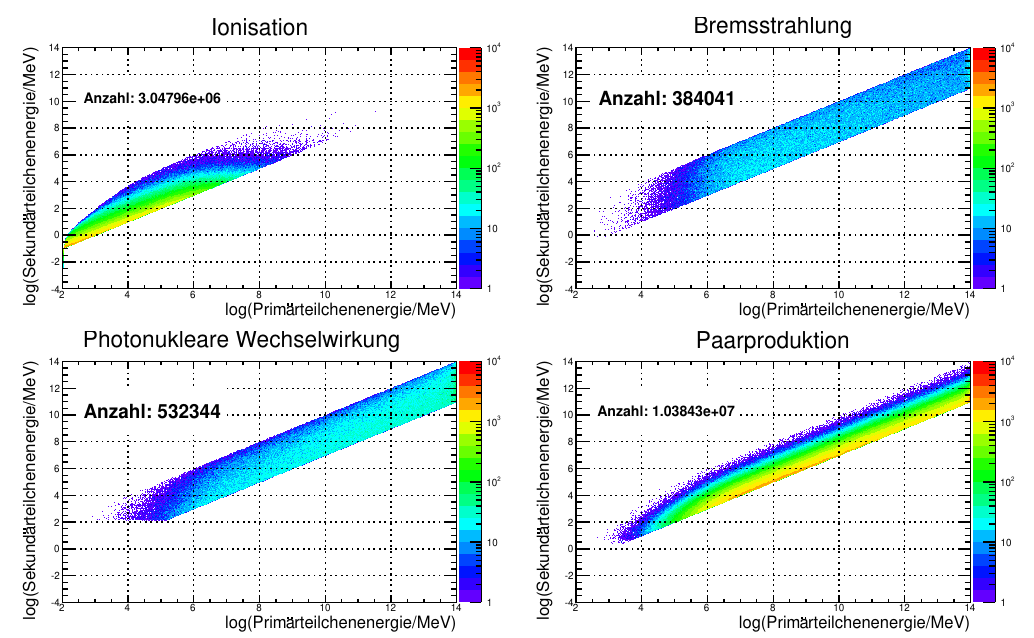
\includegraphics[width=0.7\textwidth]{plots/cut_diss_1e-3.png}
                \caption{Muon energy losses for different interaction types, using no $e_\text{cut}$ and $v_\text{cut} = \num{e-3}$.\\ \emph{From "Der Leptonpropagator PROPOSAL", Jan-Hendrik Köhne, PhD thesis 2013}}
            \end{figure}
\end{frame}

\begin{frame}
            \begin{figure}
                \centering
                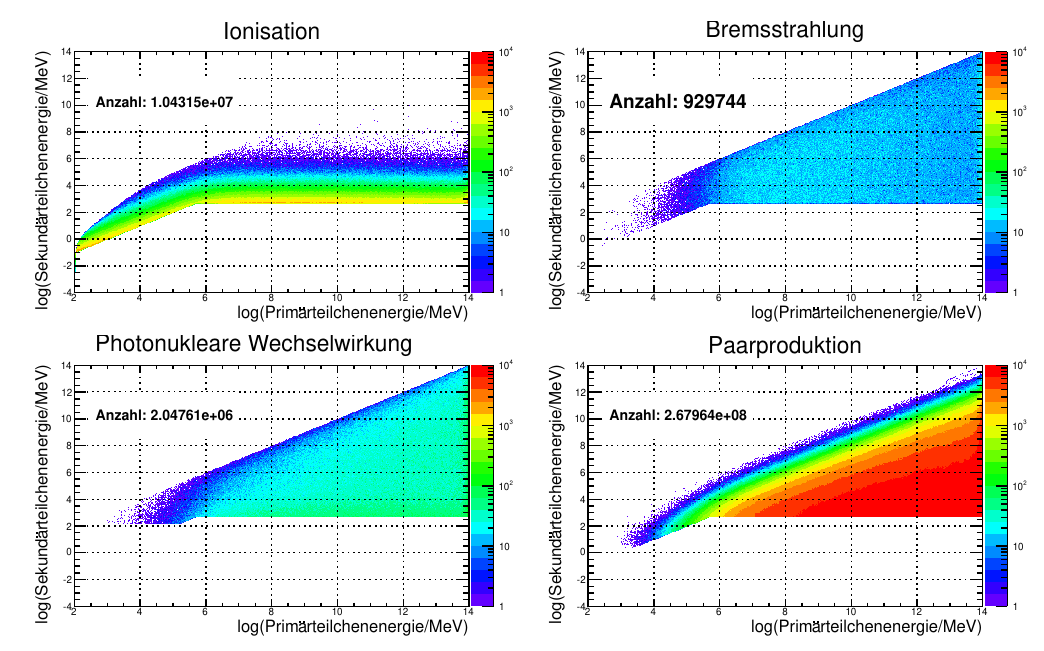
\includegraphics[width=0.7\textwidth]{plots/cut_diss_500_1e-3.png}
                \caption{Muon energy losses for different interaction types, using $e_\text{cut} = \SI{500}{\mega\electronvolt}$ and $v_\text{cut} = \num{e-3}$.\\ \emph{From "Der Leptonpropagator PROPOSAL", Jan-Hendrik Köhne, PhD thesis 2013}}
            \end{figure}
\end{frame}

\begin{frame}[plain,c,noframenumbering]
  \begin{center}
    \Huge Additional material: LPM effect
  \end{center}
\end{frame}


{
\setbeamercolor{background canvas}{bg=}
\includepdf[pages=6]{lpm_effect.pdf}
}

{
\setbeamercolor{background canvas}{bg=}
\includepdf[pages=7]{lpm_effect.pdf}
}


{
\setbeamercolor{background canvas}{bg=}
\includepdf[pages=8]{lpm_effect.pdf}
}



\end{document}

